\documentclass{article}
\usepackage{graphicx}
\usepackage[utf8]{inputenc}
\usepackage{url}
\usepackage{natbib}
\bibliographystyle{agsm}
\usepackage{float}
\usepackage{pythonhighlight}


\graphicspath{ {./images/} }

\newcommand{\quickwordcount}[1]{%
  \immediate\write18{texcount -1 -sum -merge -q #1.tex output.bbl > #1-words.sum }%
  \input{#1-words.sum} words%
}

\title{An Approach to Identify Performance Differences Based on Hausdorff Distance}

\author{Quentin Sonnefraud}
\date{July 2020}

\begin{document}

\maketitle

\tableofcontents

\section{Introduction}

This dissertation is an approach of an evolution of the RebenchDB project, which is about trying to differentiate the result from two iterations of a Programmation language implementation. 
ReBench is a tool to run and document benchmark experiments. Rebench is maintained by \cite{ReBench:2018}. In this dissertation, I'm using a side project, ReBenchDB, which is a project started in late 2019 by \cite{ReBench:2018}. The goal of ReBenchDb is to store and facilitate the analytics process with useful performance statistics of the data recorded by ReBench. Benchmark data produced from Rebench doesn't know to classify automatically if that benchmark has reached a steady-state nor if their behaviour differs from the previous iteration of the code. This dissertation will focus more on using the data provided by rebench. \\ 
The first part is about applying the work done on warmup analysis by \cite{barrett2017virtual} in order to try the result of the algorithm and see if it could work to identify and compare two benchmarks from two different iterations of the Programmation language implementation.
The second part is to review and apply a different approach to the warmup paper to quantify the behaviour or difference from the benchmark. This part will use comparison algorithms between curve to quantify the difference between two benchmarks. This comparison will quantify if a benchmark as changed in term of behaviour. In the third part, this dissertation will explain more technically how the data is managed with a PostgreSQL and node.js.\\


\section{Warmup analysis and warmup State classification (Context}

For the first expression of the need of Stefan Marr was to think about adding a feature, for his project RebenchDB. The project feature consists of trying to detect a performance difference between two versions of an algorithm. For that in this part of the dissertation I will briefly explain what is Just in Time Compilation and what consists the work done by \cite{barrett2017virtual}, then in the last part its the application in Python of the Paper with minor modifications of the algorithms that \cite{barrett2017virtual} present in their paper. We first need to define what is Just in time compilation and use and apply for the work already done by \cite{barrett2017virtual}

\subsection{What is just in time compilation? }

In order to understand the benchmark data and the work done by \cite{barrett2017virtual}, in need briefly recap what is just in time compilation.

Just in time compilation \cite{aycock2003brief} is that a concept that dynamically adapts to the current software workload, compiling "hot" code, which is the most used code at a given time (which may represent the entire program, but often only certain parts of the program are processed by Just in time compilation).

The interpreters don't have to go through all the compilation steps before they can execute anything. They start translating the first line and execute it immediately.

Because of this, an interpreter naturally seems to be a good choice to run something like JavaScript. It is important for a web developer to be able to start executing his code as fast as possible. That's why browsers have used interpreters to run JavaScript in the beginning.
The problem with interpreters occurs when you want to run the same code more than once. Typically when you use a loop. In this case, the interpreter has to do the same translation over and over again.

A compiler chooses the opposite compromises.

It needs a little more time at startup because it has to go through all the compilation steps before it can do anything. However, executing the code in a loop is much faster because it is no longer necessary to redo the translation work each time it passes through the loop.
Another difference is that compilers have more time to observe the code and modify it so that it can run faster. These modifications are nothing more and nothing less than optimizations. Since the interpreters do the translation work at the same time as they run the code, they cannot afford to take much time to make optimizations.

In order to overcome the inefficiency of interpreters - having to translate the same code over and over again - browsers have started to add compilers to them.

Each computer and compiler does this in a slightly different way, but the basic idea remains the same. A new piece is added to the Language engine: a code profiler. This profiler observes the code as it runs and makes notes on how many times a piece of code is executed and what types are used.

At first, the profiler runs everything through the interpreter.

If the same lines of code are executed a few times, this piece of code is considered "warm". If it is executed very often, it is considered "hot".

When a function becomes lukewarm, the JIT will send it to the compiler and will store the result of the compilation.

The basic compiler (BC for Baseline Compiler)

Each line of code is compiled as a "chunk". Extracts are indexed by line number and by variable type. If the profiler notices that the same code with the same variable types is executed again, it will simply use the compiled stub.

This helps speed things up. But as I said, a compiler can do much more. It can take the time to figure out the most efficient way to do certain things to make optimizations. The basic compiler will do some of these optimizations. This should not take too much time, because it doesn't want to freeze the execution for too long.

However, if this code is really hot if it is executed really often, then it is worth taking the time to do more optimizations.

Those warm and hot phases are what \cite{barrett2017virtual} are interested in. Indeed they record every performance for a lot of algorithms. They wrote an algorithm which identifies if those warm and hot phase is really speeding up the code. This warm and hot phase can help us with the classification of a performance difference.

\cite{barrett2017virtual} used krun, which is an extreme benchmark runner which prepares the machine and the operating system for performing precise measurements of computer programs. It is kind of similar Rebench because it records some benchmarking data.

\subsection{Background work on Warmup Phase Classification}

.
For this dissertation work, I implemented a study of \cite{barrett2017virtual} about characterizing warmup stages of popular virtual machines (VM), HHVM (PHP), Graal, HotSpot JVM (java), and others. 
In the study, various benchmarks were repeatedly executed on each virtual machine to see when the JIT compilation happens and how it affects the performance.
They have observed that JIT compilation usually increases the program performance; however, in very some cases, it might even lead to performance degradation or no steady-state for the programme. Moreover, I have observed the JIT compilation happens mostly during the first run of a program, which indicates that a "warmup phase".
In \cite{barrett2017virtual} Papers for benchmark states classification, they used three steps.

\begin{itemize}
    \item The first step is to clean outliers such as garbage collection or JIT compilation as seen above. A garbage collector is a computer subsystem for automatic memory management.  It is responsible for recycling previously allocated and unused memory.  
    \item The second step after cleaning those outliers from the data is to applied a change-point algorithm \cite{killick2014changepoint}
    \item The third step After getting the breakpoints from the change-points algorithm is to have each segment of the experiments and pass them to the classification algorithm that \cite{barrett2017virtual} have made which will classify the experiment with four class (warmup, flat, slow down or no steady-state).
\end{itemize}




\subsection{Clean outliers}

As with the analysis of time-series data, They had first mostly determined the outliers ( much larger / pretty much smaller than close neighbours). In the paper \cite{barrett2017virtual} they said that this data, can particularly be compile-time of JIT, Garbage collection or basically other processes that specifically do specifically interfere with the benchmarks in a subtle way. I applied the same techniques of \cite{barrett2017virtual} to get the same results which, for the most part, is a rolling window to remove the outliers in the benchmarks like the garbage collection in an actually major way.

\begin{figure}[h!]
    \centering
    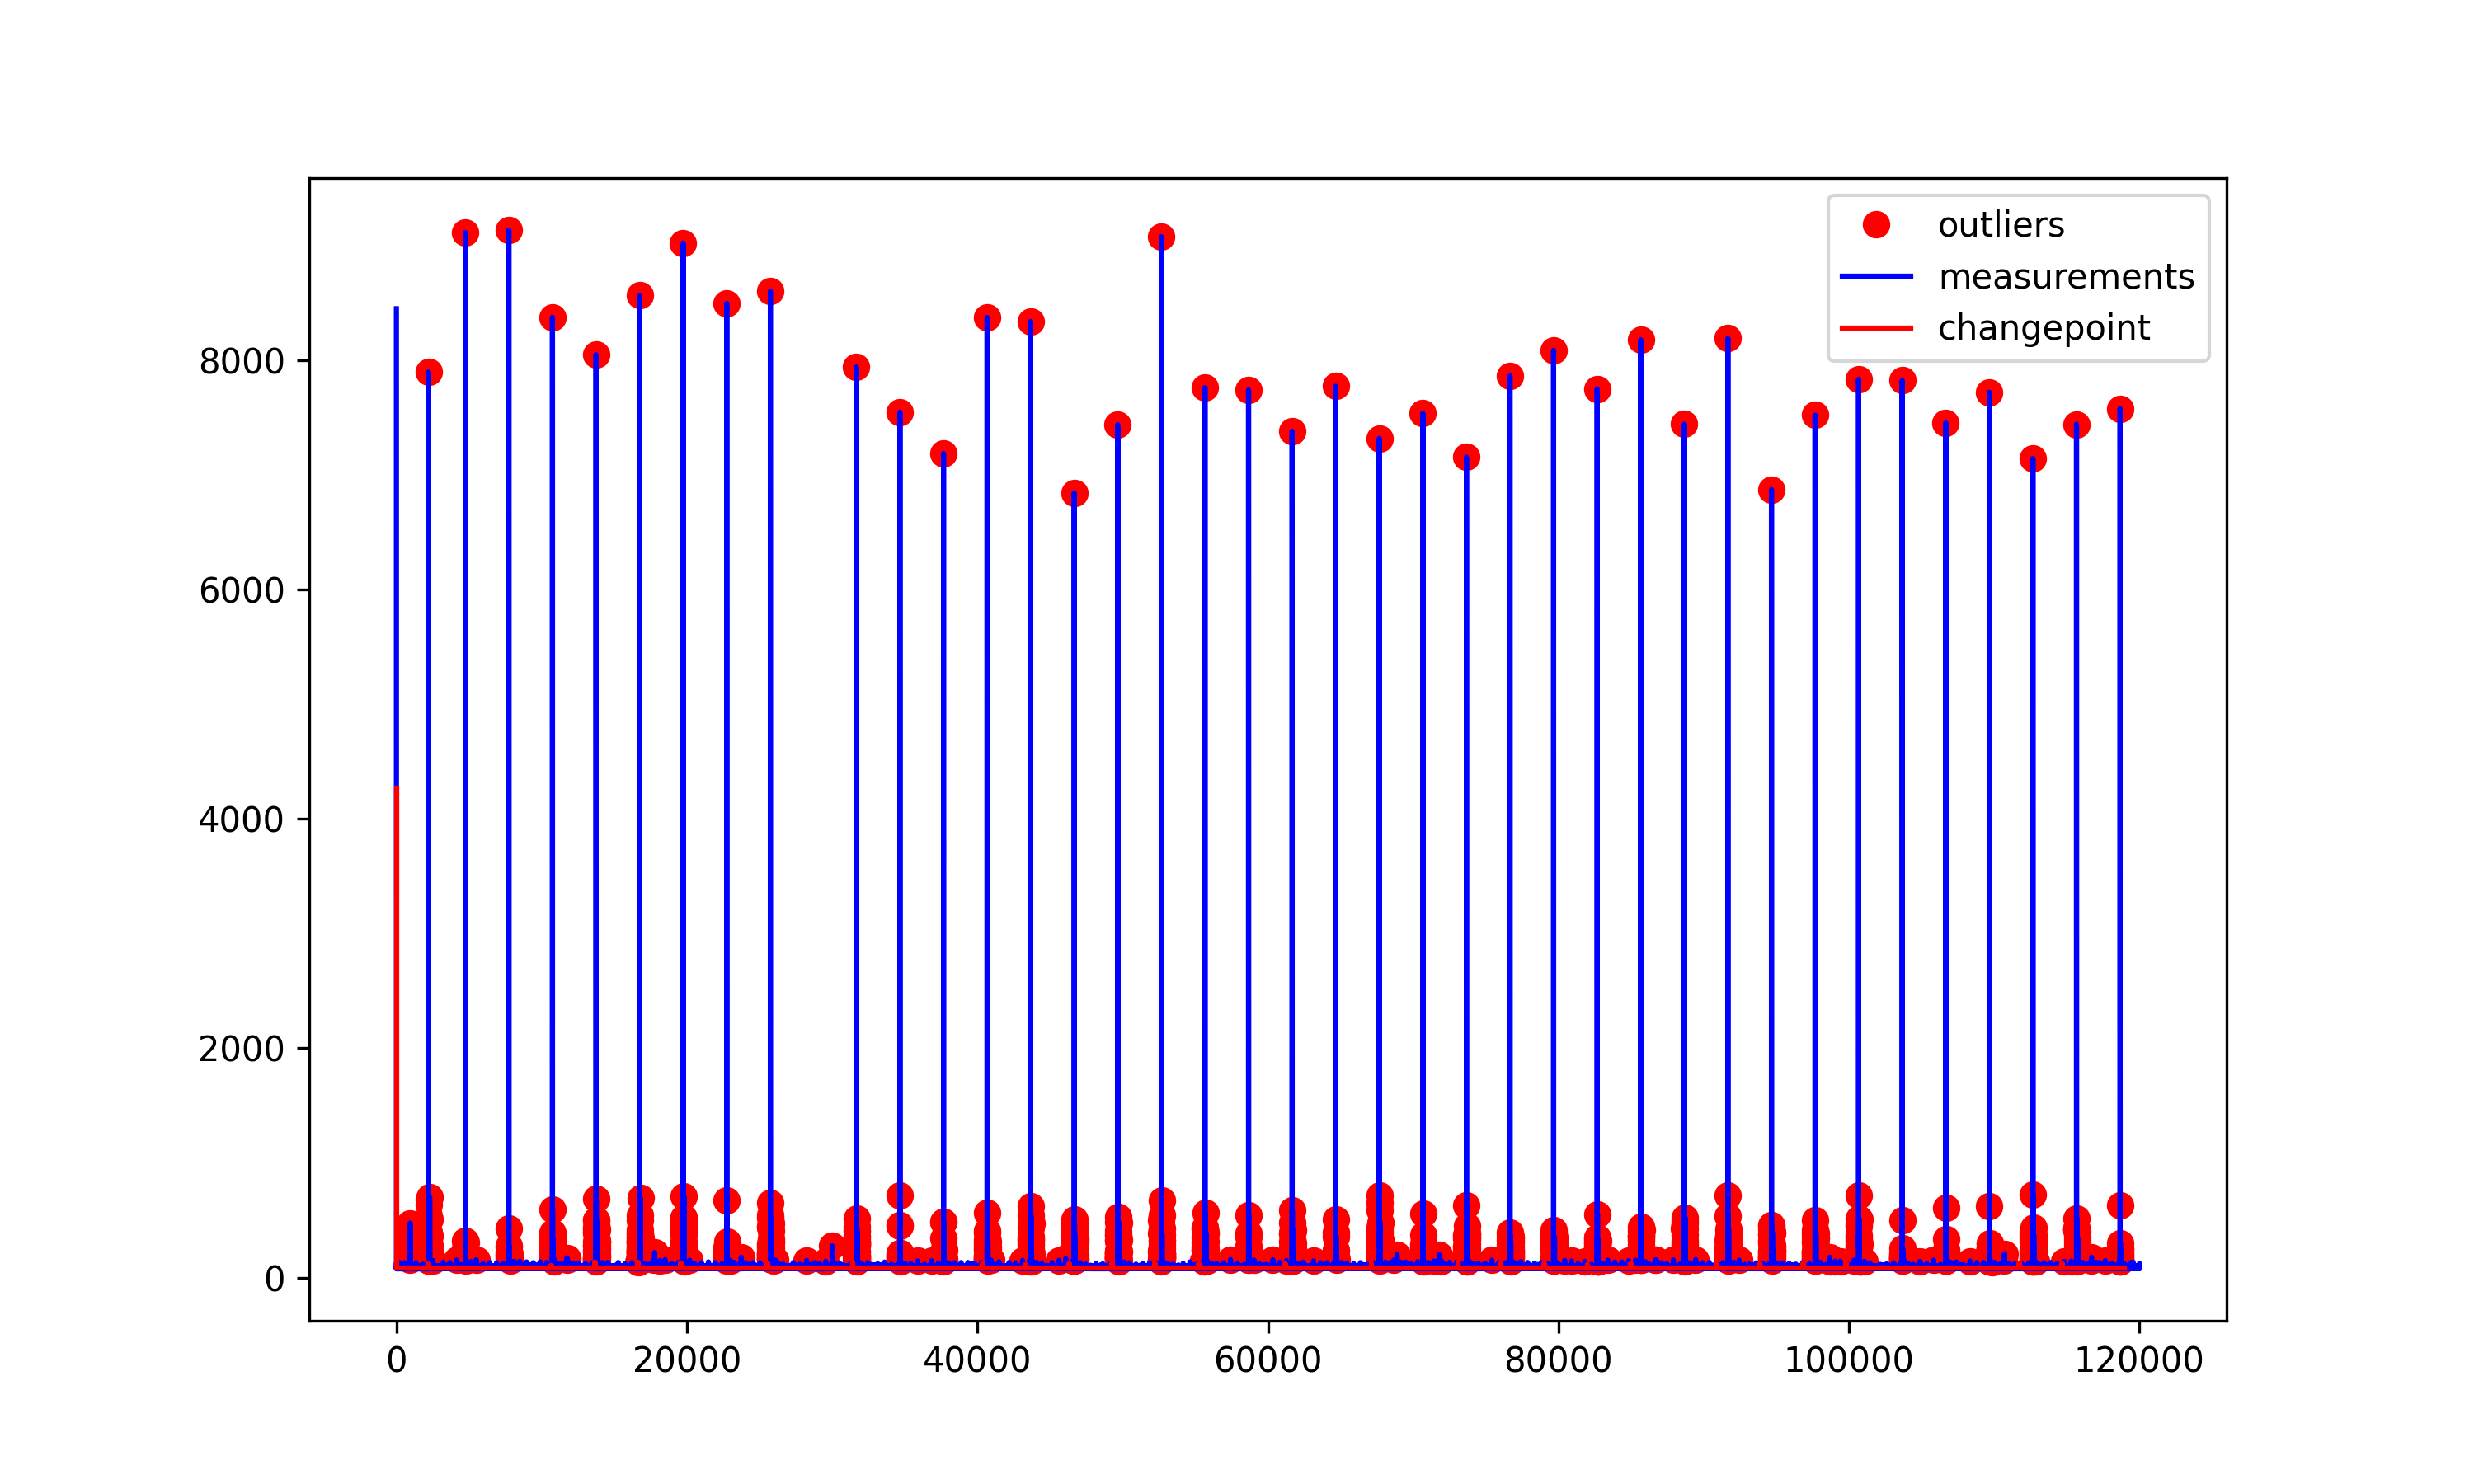
\includegraphics[width=1\textwidth]{images/plot_13_flat.png}
    \caption{CD benchmark from Node classify as warmup affected mostly in means}
    \label{fig:bench_node_flat}
\end{figure}

For example, the problem here from the previous techniques with rolling window is that it doesn't remove the first outliers because it ignores the 200 first measurements, but you could have some outliers in this part of the measurements. So I'm trying to find a better technique to remove those outliers.

Anomaly detection consists in highlighting data with different behaviour from the majority of the data. 
Indeed, the detection can be performed in a supervised mode in case information on the normality of the data is available which is not the case here because it would mean to label the outlier inside the rebench data. In other words, any data in the learning base can be labelled as normal or abnormal.
As for the detection in unsupervised mode, no information on the normality of the data is available which the case here and the case in the \cite{barrett2017virtual} paper and for the rebench data. 

\subsubsection{Unsupervised techniques}
The unsupervised approach is the most suitable for anomaly detection problems and benchmarks data. In this approach, the different algorithms try to distinguish aberrant observations by learning about the data set, without having the labels of the observations: there is no set of observations identified a priori as anomalies. It is therefore not necessary to have labelled data, and this simplifies the problem of preparing the data before learning and all the difficulty in constructing labels.

In the paper they apply the rolling window by removing all elements that are outside the mean by 15\% and 85\% They ignore the 200 measurements because it would remove too much interesting data about warmup which represent 10\% of the size of the whole benchmark in their paper. There was some problem with outlier removing because in the rebench data there was clearly outlier that past the warmup phase should be removed, so I reduced the ignore phase to 5\% (100 first measurements for a benchmark of 2000 measurements which are ignored).



\subsection{Overview of Changepoint detection algorithm}


So first I used a package which allows me to do changepoint analysis which is called ruptures \cite{truong2020selective}, it works well, but after reading the warmup paper I prefer to use the algorithm from R "changepoint" \cite{killick2014changepoint} in order to reproduce the experiment.



\subsection{Changepoint Detection}
In statistical analysis, the changepoint detection problem is a regression problem to estimate the times at which a signal exhibits changes in the distribution. Classically, changepoint detection is performed for a signal with changes in the mean. More generally, changepoint detection is performed for a signal with changes in the distribution (for example, in the mean and variance). \\

Changepoint detection can be applied to a sound signal of a program for which we wish to estimate the moments when situations change, to the detection of computer attacks, or to quality control, here for the rebench data it helps to classify behaviour in warmup analysis. \\

This next will deals with the problem of detecting changepoint retrospectively (known as offline) when all the signal data are available. This context is different from a real-time detection (online) where the signal data arrive on the fly it could be interesting to classify on the fly after reaching and classifying a stabilization of a benchmark and stoping recording the benchmark data in order to save time, but online detection is less able to detect precisely the moment of rupture.

\subsection{Offline detection Parametric and Non Parametric}
 
 
There two big families of the offline detection algorithm.

\subsubsection{Parametric}

Advantages: speed of calculation, ease of interpretation and prediction,
good speed of convergence, the possibility of validation;
Disadvantages: a priori choice of known functions (for example the degree of polynomial), adapted to a limited class of tendencies.

\subsubsection{Non-parametric}

\begin{itemize}
    \item Advantages: adaptability, not a priori on the type of trend;
    \item Disadvantages: limits in interpretation, validation and prediction, choice of window / smoothing parameters.
\end{itemize}

Of course, there are very different ways of proceeding to analyze this type of signal. One of the most "intuitive" is to cut the series into "homogeneous" segments. This notion of homogeneity can cover, for example, homogeneity in mean, or homogeneity in variance (or homogeneity in mean-variance!).

There is 3 type of detection of Changepoint.

Changepoint in mean, Changepoint in variance, and Changepoint mean or variance.

In the paper \cite{barrett2017virtual} They used mean and variance detection with the changepoint algorithm.



\begin{figure}[h!]
    \centering
    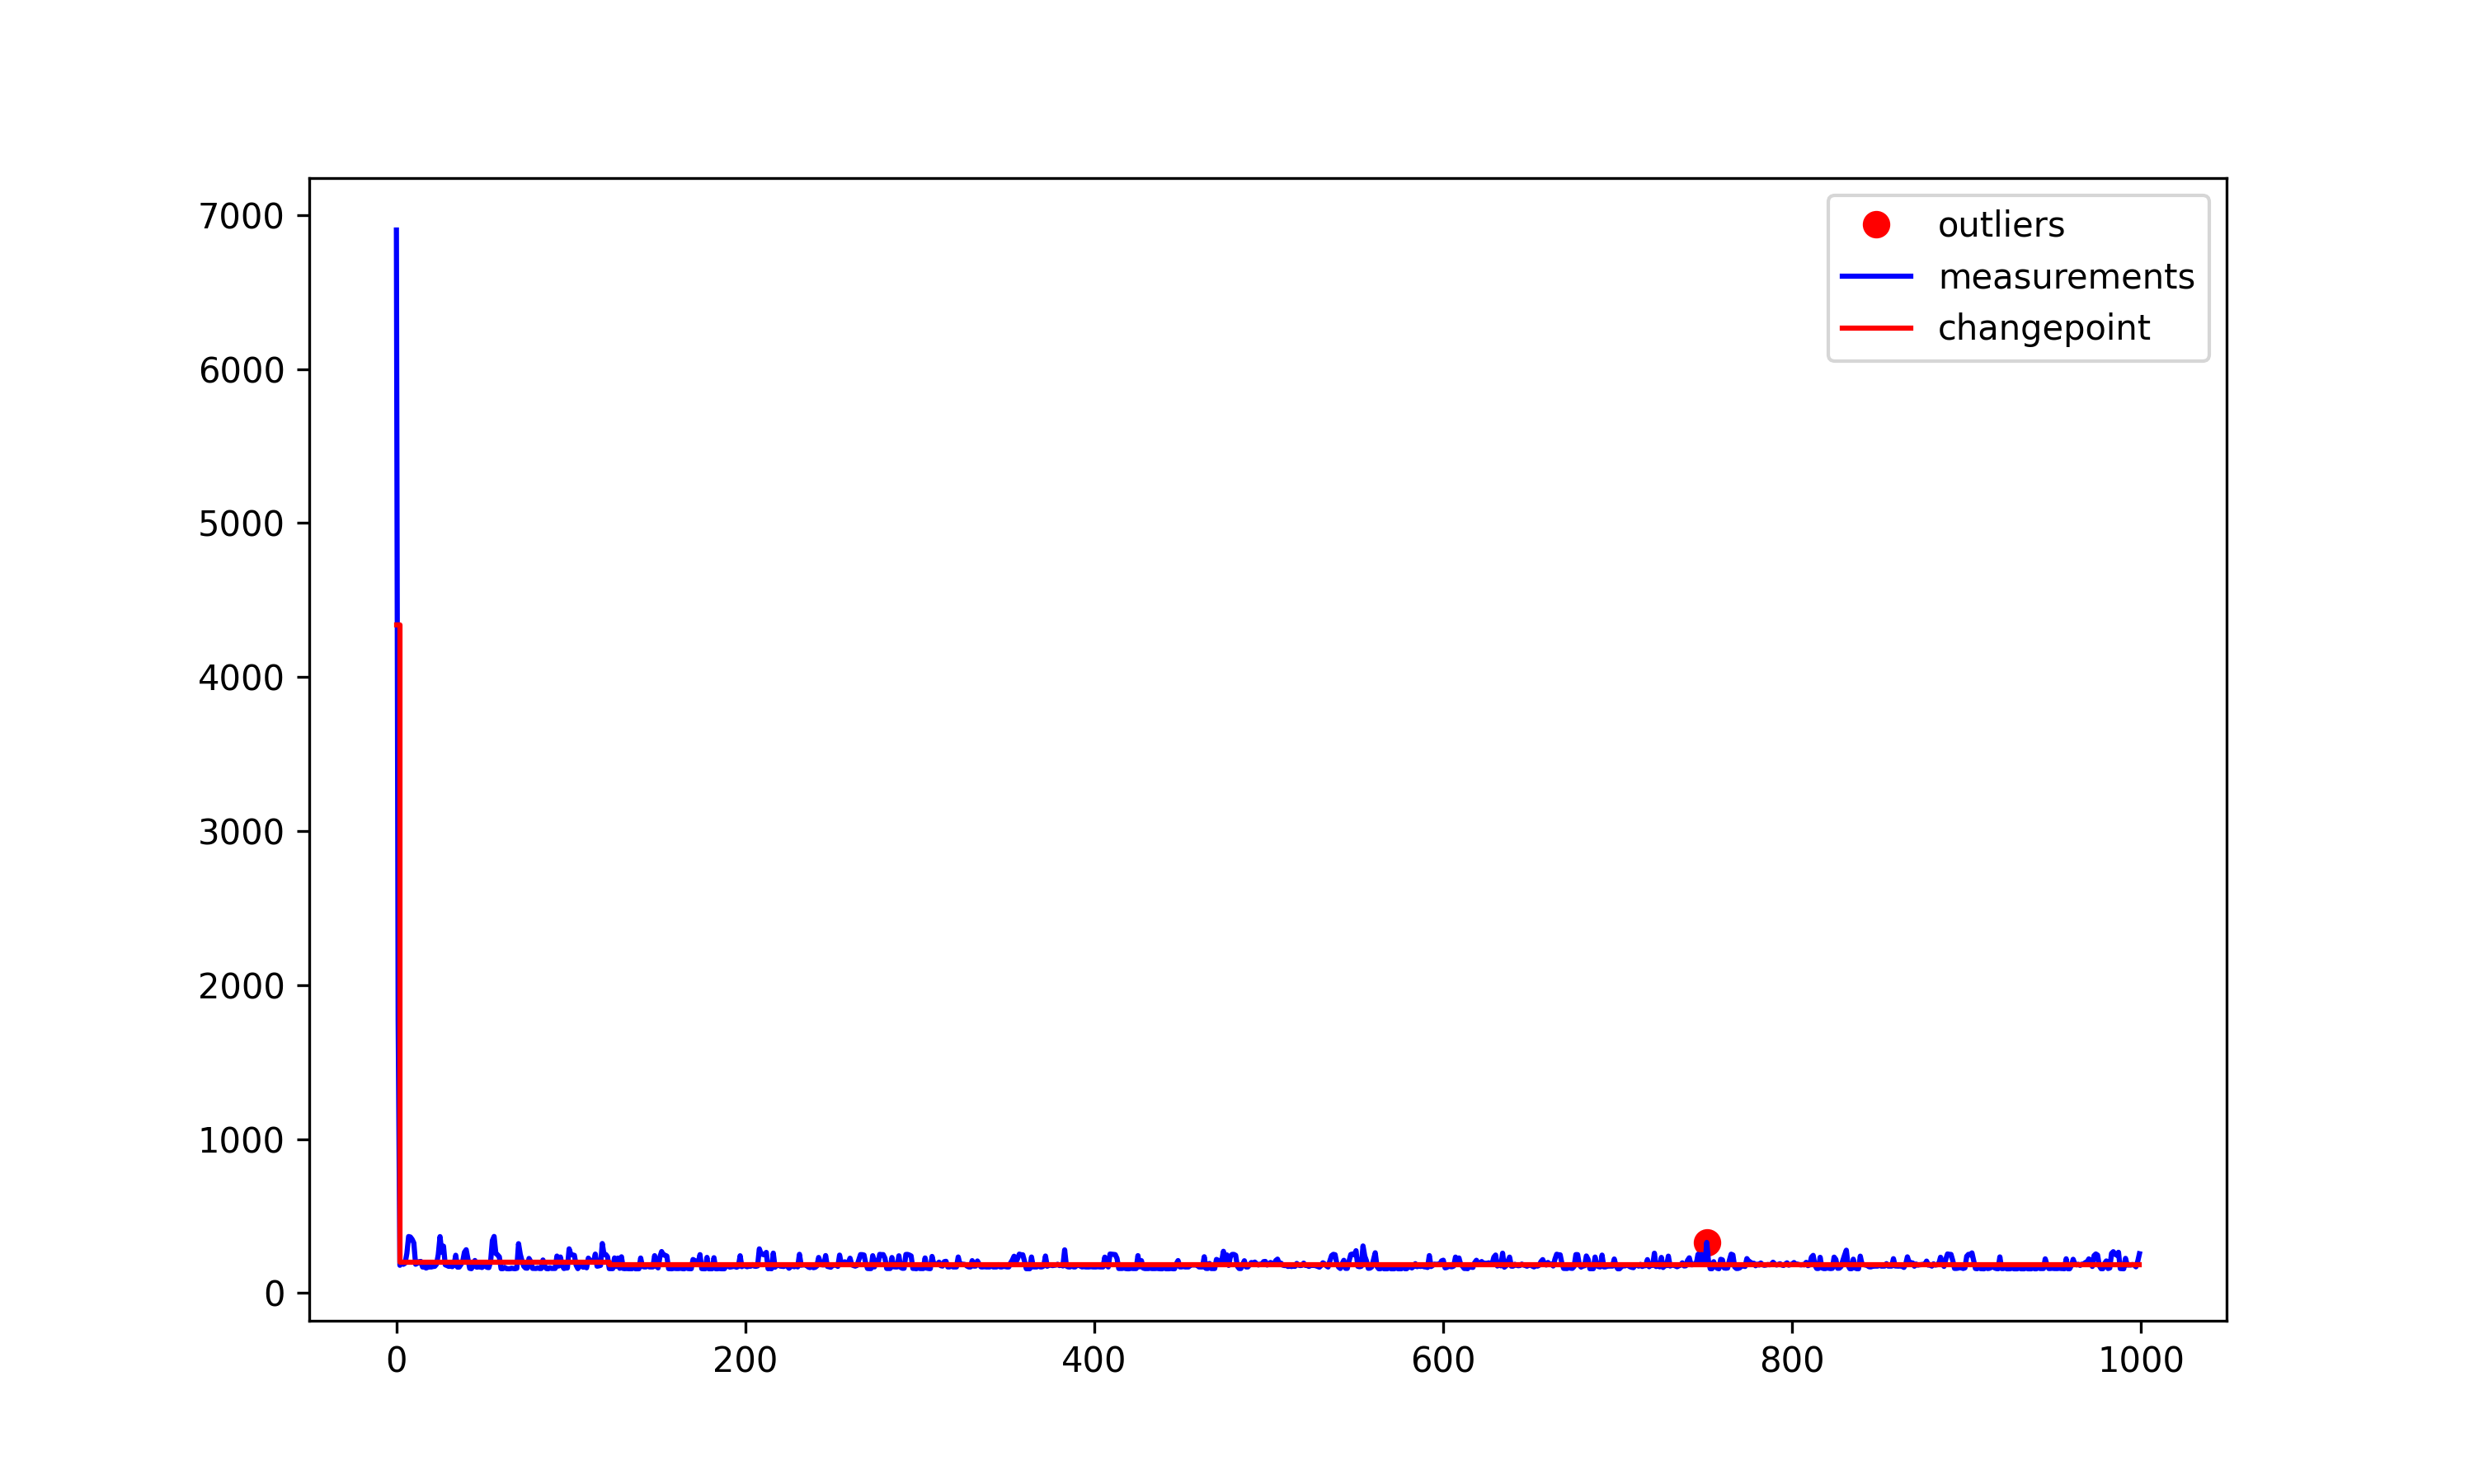
\includegraphics[width=1\textwidth]{images/plot_6_flat.png}
    \caption{CD benchmark from Node classify as warmup affected mostly in means}
    \label{fig:bench_node_flat}
\end{figure}



\begin{figure}[h!]
    \centering
    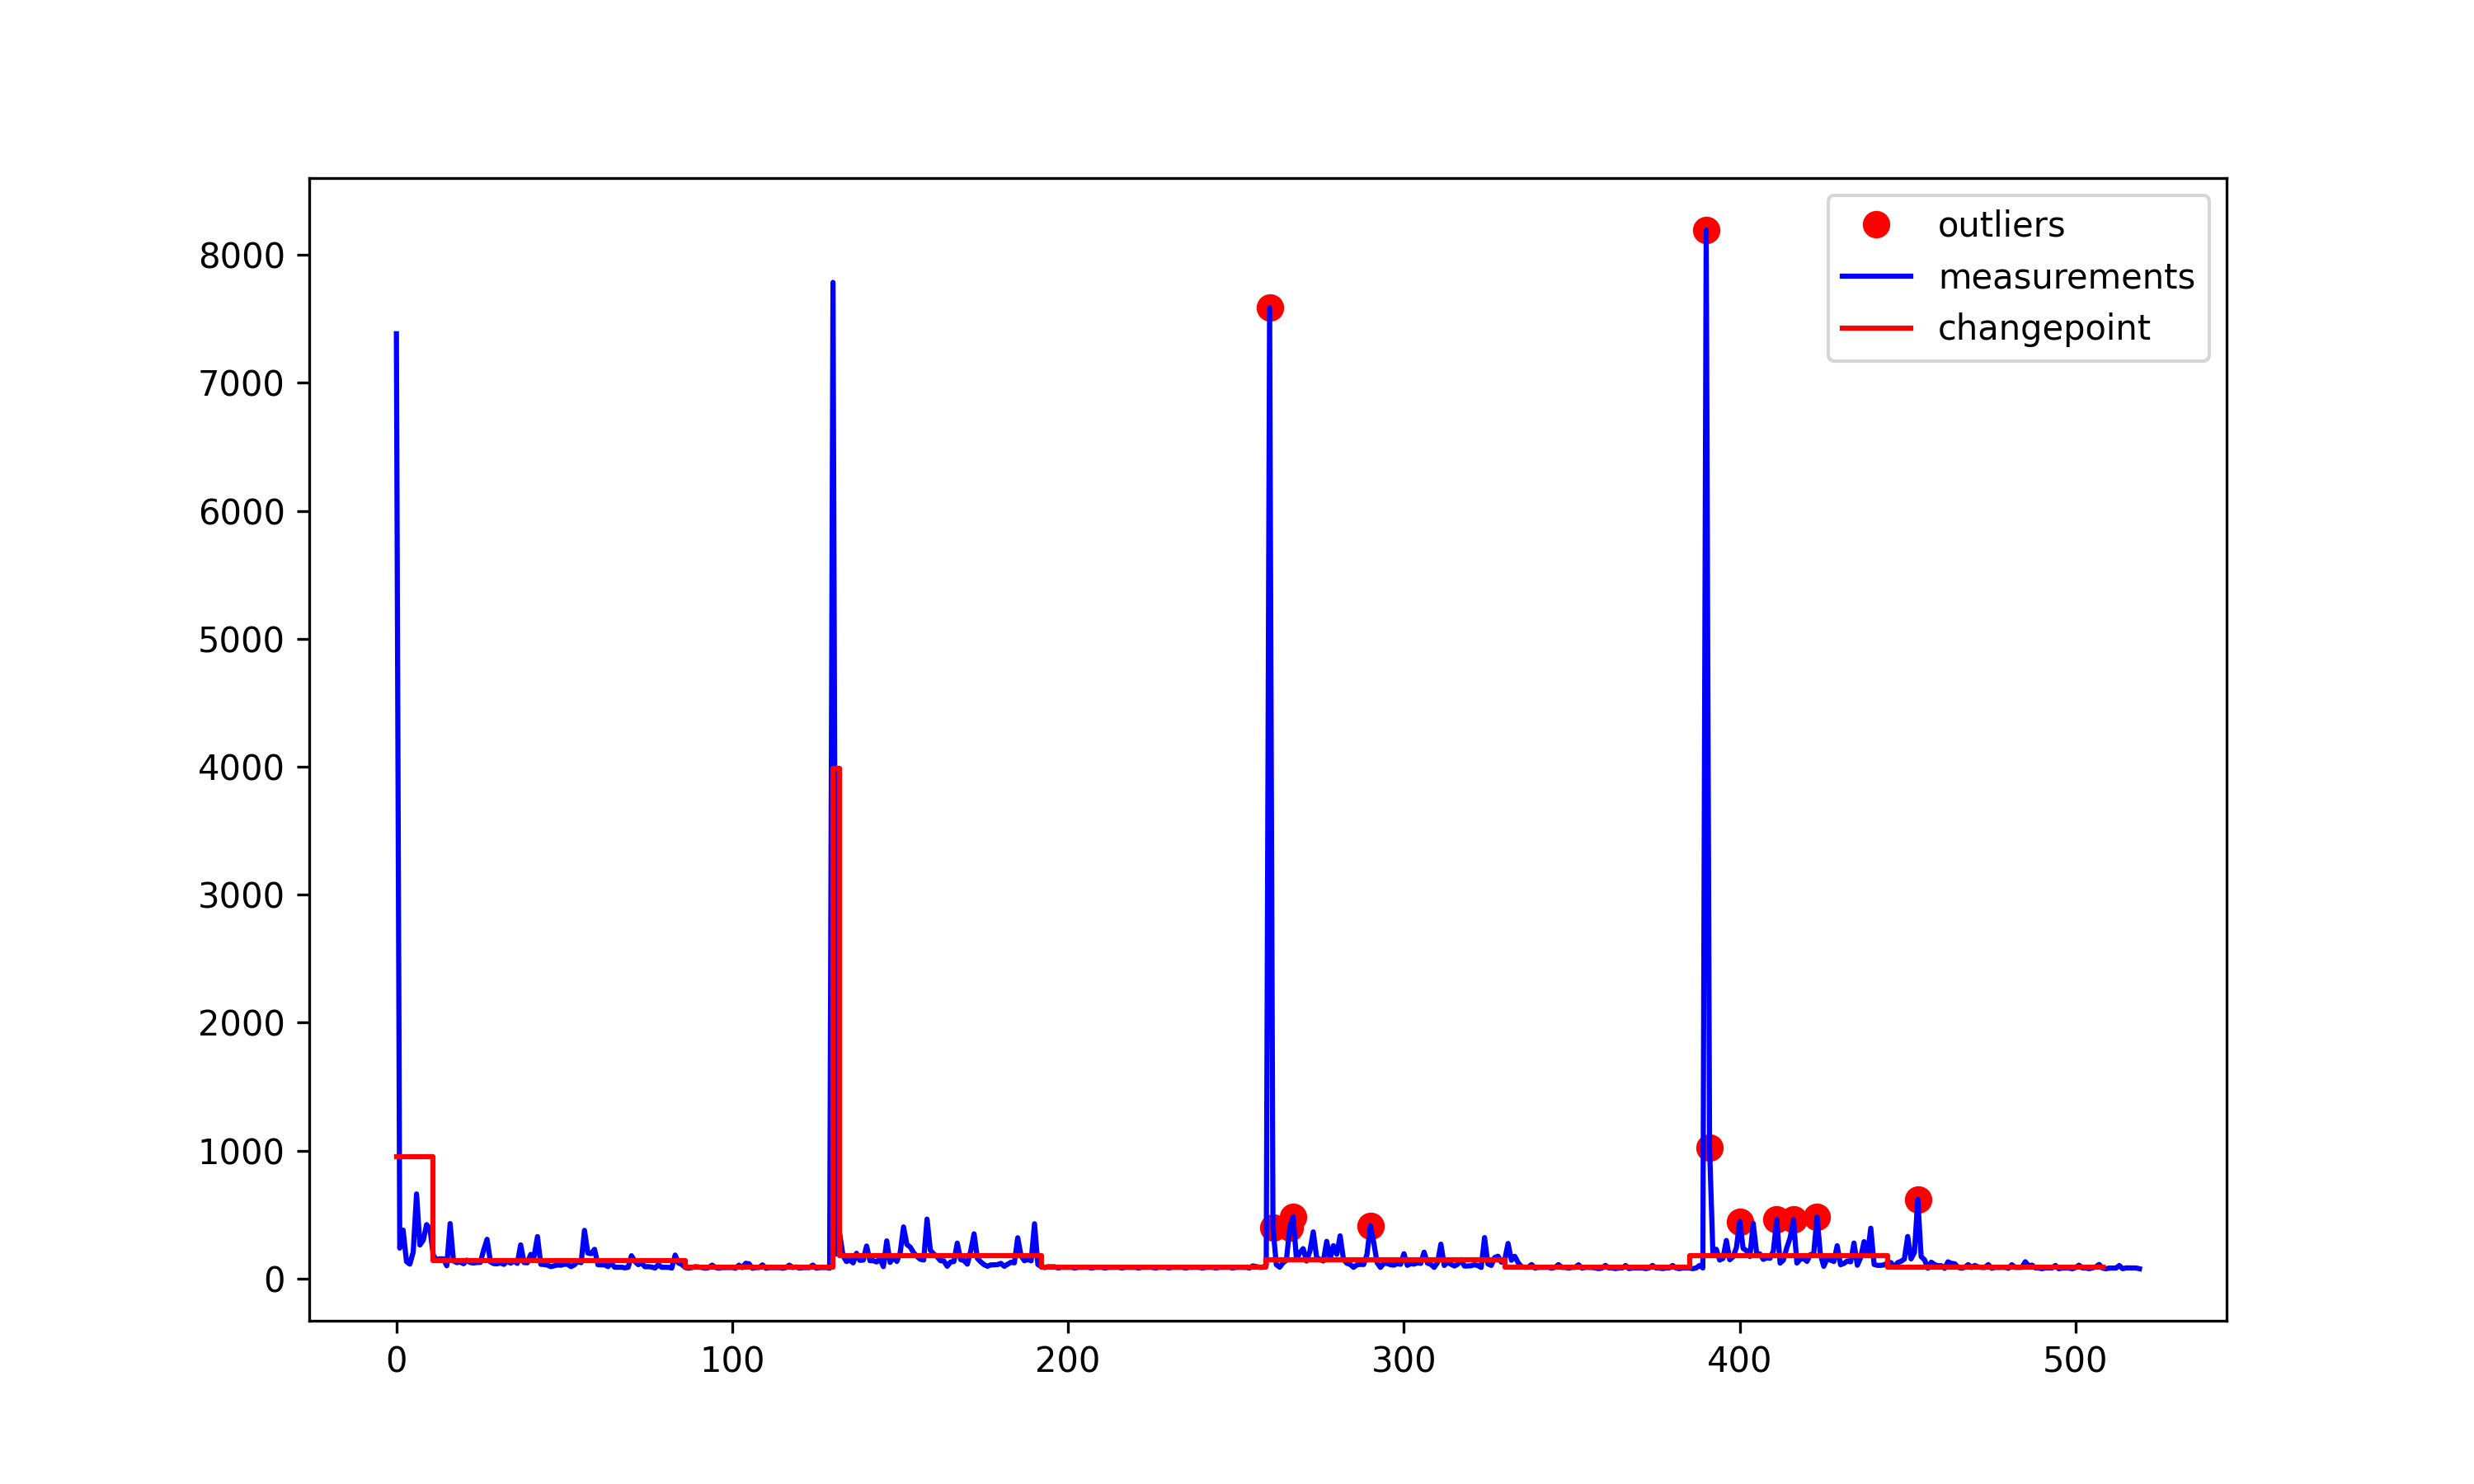
\includegraphics[width=1\textwidth]{images/plot_10_flat.png}
    \caption{CD benchmark from SOMns classify as warmup affected mostly in means and variance}
    \label{fig:bench_somns_flat}
\end{figure}

For example, for the two benchmarks above, it looks like:

the \ref{fig:bench_node_flat} series is affected by changes in the average,
the \ref{fig:bench_somns_flat} series by changes in mean and variance.


Based on these models, here is the kind of segmentation that could be proposed:

The above results are actually obtained using the changepoint package from \cite{killick2014changepoint}.

In the warmup paper, they discussed three different functions:

cpt.mean which is used to detect changepoint in the mean (assuming that the variance is constant)
cpt.var which is used to detect  in the variance (assuming that the mean is constant)
cpt.meanvar which is used to detect changepoint in both the mean and the variance
These three functions are largely configurable. One can thus vary (among others)

The nature of the algorithm used to detect "optimal" breakpoints...
the type of test used to locate the changepoint (one can either assume that the residual distribution of the variables is Gaussian, or one can not make an assumption of distribution and use a non-parametric test)
the type and extent of the penalty applied in order to limit over-segmentation.

These aspects are discussed in \cite{killick2014changepoint}.

\subsection{Effect of parameterization}

Unsurprisingly, the above functions give very different results depending on how you set them up.

To choose the segmentation algorithm and other associated parameters, we will rely on three criteria:

Theoretical criteria (which model is best suited to the data? one with constant variance, one where the residuals are Gaussian, one that would account for segments of highly variable lengths, etc.).

Empirical criteria (I choose the method that gives the most "usable" results on real the warmup paper, and the correct results on the data from rebench data). This is what I used because I assume that the data and the result of the classification from \cite{barrett2017virtual} were verified and are correct.

Calculation criteria (the method must be computationally applicable for data of a certain size).

Obviously, determining which method is best using multiple criteria of these three types is difficult. Nevertheless, it is possible to discuss it by carrying out the same type of study as \cite{leviandier2012comparison}. This could be a future work to find the best parameters for changepoint analysis for rebench data and/or \cite{barrett2017virtual} paper but for this experiment, I will stick to the parameters they used in the warmup paper.

\subsection{Classification}


There was some problem with the classification I adapted the algorithm which works now depending on the size of the benchmarks.
The classify function from \cite{barrett2017virtual} takes as parameters the measurements from rebench and the length of the measurements it is useful because otherwise, the STEADY\_STATE\_LEN would stay to 500 which is not suitable when the length of the measures are under 500 for example. After all, it would mean that the steady-state length would be more than the size of measurements which is not possible.

This code bellow is majorly from the \cite{barrett2017virtual} but is adapted in Python and vary the classification dynamically depending on the size of the whole benchmarks.
\begin{python}[h!]

# From paper Virtual Machine Warmup Blows Hot and Cold

import NumPy as np


DELTA = 1  # Absolute time delta (in seconds) below which segments are
# considered equivalent.
STEADY_STATE_LEN = 500  # How many in-process iterations from the end of the time-series
Will # data a non-equivalent segment trigger "no steady state"?


def percentage(percent, whole):
    return int((percent * whole) / 100.0)


def classify(segs, n_values):
    assert(len(segs) > 0)
    last_seg = segs[-1]
    STEADY_STATE_LEN = percentage(25, n_values) # Steady state when the data need to stabilize
    lower_bound = last_seg['mean'] - max(last_seg['variance'], DELTA)
    upper_bound = last_seg['mean'] + max(last_seg['variance'], DELTA)
    label = "flat"
    i = len(segs) - 2
    while i > - 1:
        seg = segs[i]
        i -= 1
        if seg['mean'] + seg['variance'] >= lower_bound and seg['mean'] - seg['variance'] <= upper_bound:
            continue
        elif seg['end'] > n_values - STEADY_STATE_LEN:
            label = "no steady state"
            break
        elif seg['mean'] < lower_bound:
            label = "slowdown"
            break
        assert(seg['mean'] > upper_bound)
        label = "warmup"
    return label
\end{python}

You can see the result of this algorithm in the zip file (the corpus of the dissertation) it produced an image with the outliers and the classification given inside the filename.
The major problem to differentiate the behaviour of benchmark of this technique is that it removes a lot of information you can have totally the same behaviour from the classification for example 2 benchmarks classify as "warmup", but it will not reflect the reality because they can be classified as warmup but the curve means can be much higher compare to other which need to be considered. So I have to find other technique, and for that, I used some other techniques already used on the industry for compared directly curve by quantifying them.



\subsection{Problem for performance difference}

The main problem to identify performance difference with these techniques is that it only classifies warmup state and not perform as the whole. Based on this approach, I decided to reuse the outliers cleaning but applying another algorithm to try to differentiate performance difference. For example for figure \ref{fig:bench_node_flat} and \ref{fig:bench_somns_flat} they are both classified as flat indeed is not significant to say that those curves are the same/different We need another approach and for that, I am investigating algorithm used in curve analysis and more particularly curve comparison.




\section{ How to detect the change between benchmarks? Overview of the method to quantify the difference between curve}

During this project, I have reviewed and try some techniques to quantify the difference between benchmarks and report if Changement of behaviour as occurs. During this dissertation, I prefer to pick one benchmark problem, which is the sleeping barber algorithm \cite{reynolds2002linda}, which is a sharing resources problem in multi-tasking. The next subsection will be about explaining what is the sleeping algorithm and explaining why I am getting that kind of plot.

\subsection{Sleeping Barber problem}

The program will have to be decomposed into two types of threads. On one side there will be the barber, represented by a single thread looping continuously to see if a customer is waiting, take care of him if necessary or go to bed. On the other side, there will be one thread per client, which will simulate the "physical" client. He will try to enter the shop, sit down and if he can, get a shave. And at the end leave the shop and disappear.
While the program will have only one barber, there may be as many customers as there is memory on the computer. The client threads will, therefore, pile up, waiting for space to become available in the waiting room, and then the barber will take care of them. There are many threads that the computer allow or the user allows them to.

\subsubsection{ What does the barber do?}
The thread symbolizing the barber will, therefore, be unique so one barber equal one thread. It will be started when the program is launched, before any customer, and will loop back on itself for all eternity.
Here's what our barber will spend his life doing:

\begin{itemize}
    \item Is there anyone in the waiting room? If there is, I'll take care of him, and if not, I'll go to bed;
    \item When a customer is there I take him to the chair;
    \item I shave him;
    \item I give him the day off.
    \item Of course, when we get to the end, we loop back in.
\end{itemize}

\subsubsection{ What does the customer do?}

Here are the actions that the thread symbolizing each customer will perform. If there are several customers, identical threads will compete with each other:

\begin{itemize}
    \item I look in the hairdressing salon to see if there's any free space. If there is, I go inside, if not, I wait;
    \item When I'm inside I sit on a chair (and take my comic);
    \item I wait until the barber is free;
    \item I get up from my chair (and free a seat) and go into the room;
    \item I let myself trim my beard;
    \item When he's done, I pay and go home.
\end{itemize}

Looking at the difference in the number of tasks between the barber's and the client's list of actions, we notice that the client does more things. In fact, the client has to manage an additional resource compared to the barber: the free place in the waiting room when he comes to the entrance of the salon. On the benchmarks from the sleeping barber experiments, you can get some kind of step which you can identify as when the algorithm used the maximum of the threads, and that can explain the poor performance of the algorithm. And when the step is lower that's means there is not so much task going tr ought the algorithm.

\subsection{Benchmarks data from Sleeping Barber experiment}

For running the comparison between two curves, I chose four iterations of the experiments of the sleeping barber problem implementation. The first one is a record one thousand iteration of the benchmarks and the second and the third one are a record of 5500 iterations there are from the project SOMNS, which is an implementation of the Newspeak Specification derived from the Simple Object Machine,

\begin{figure}[h!]
    \centering
    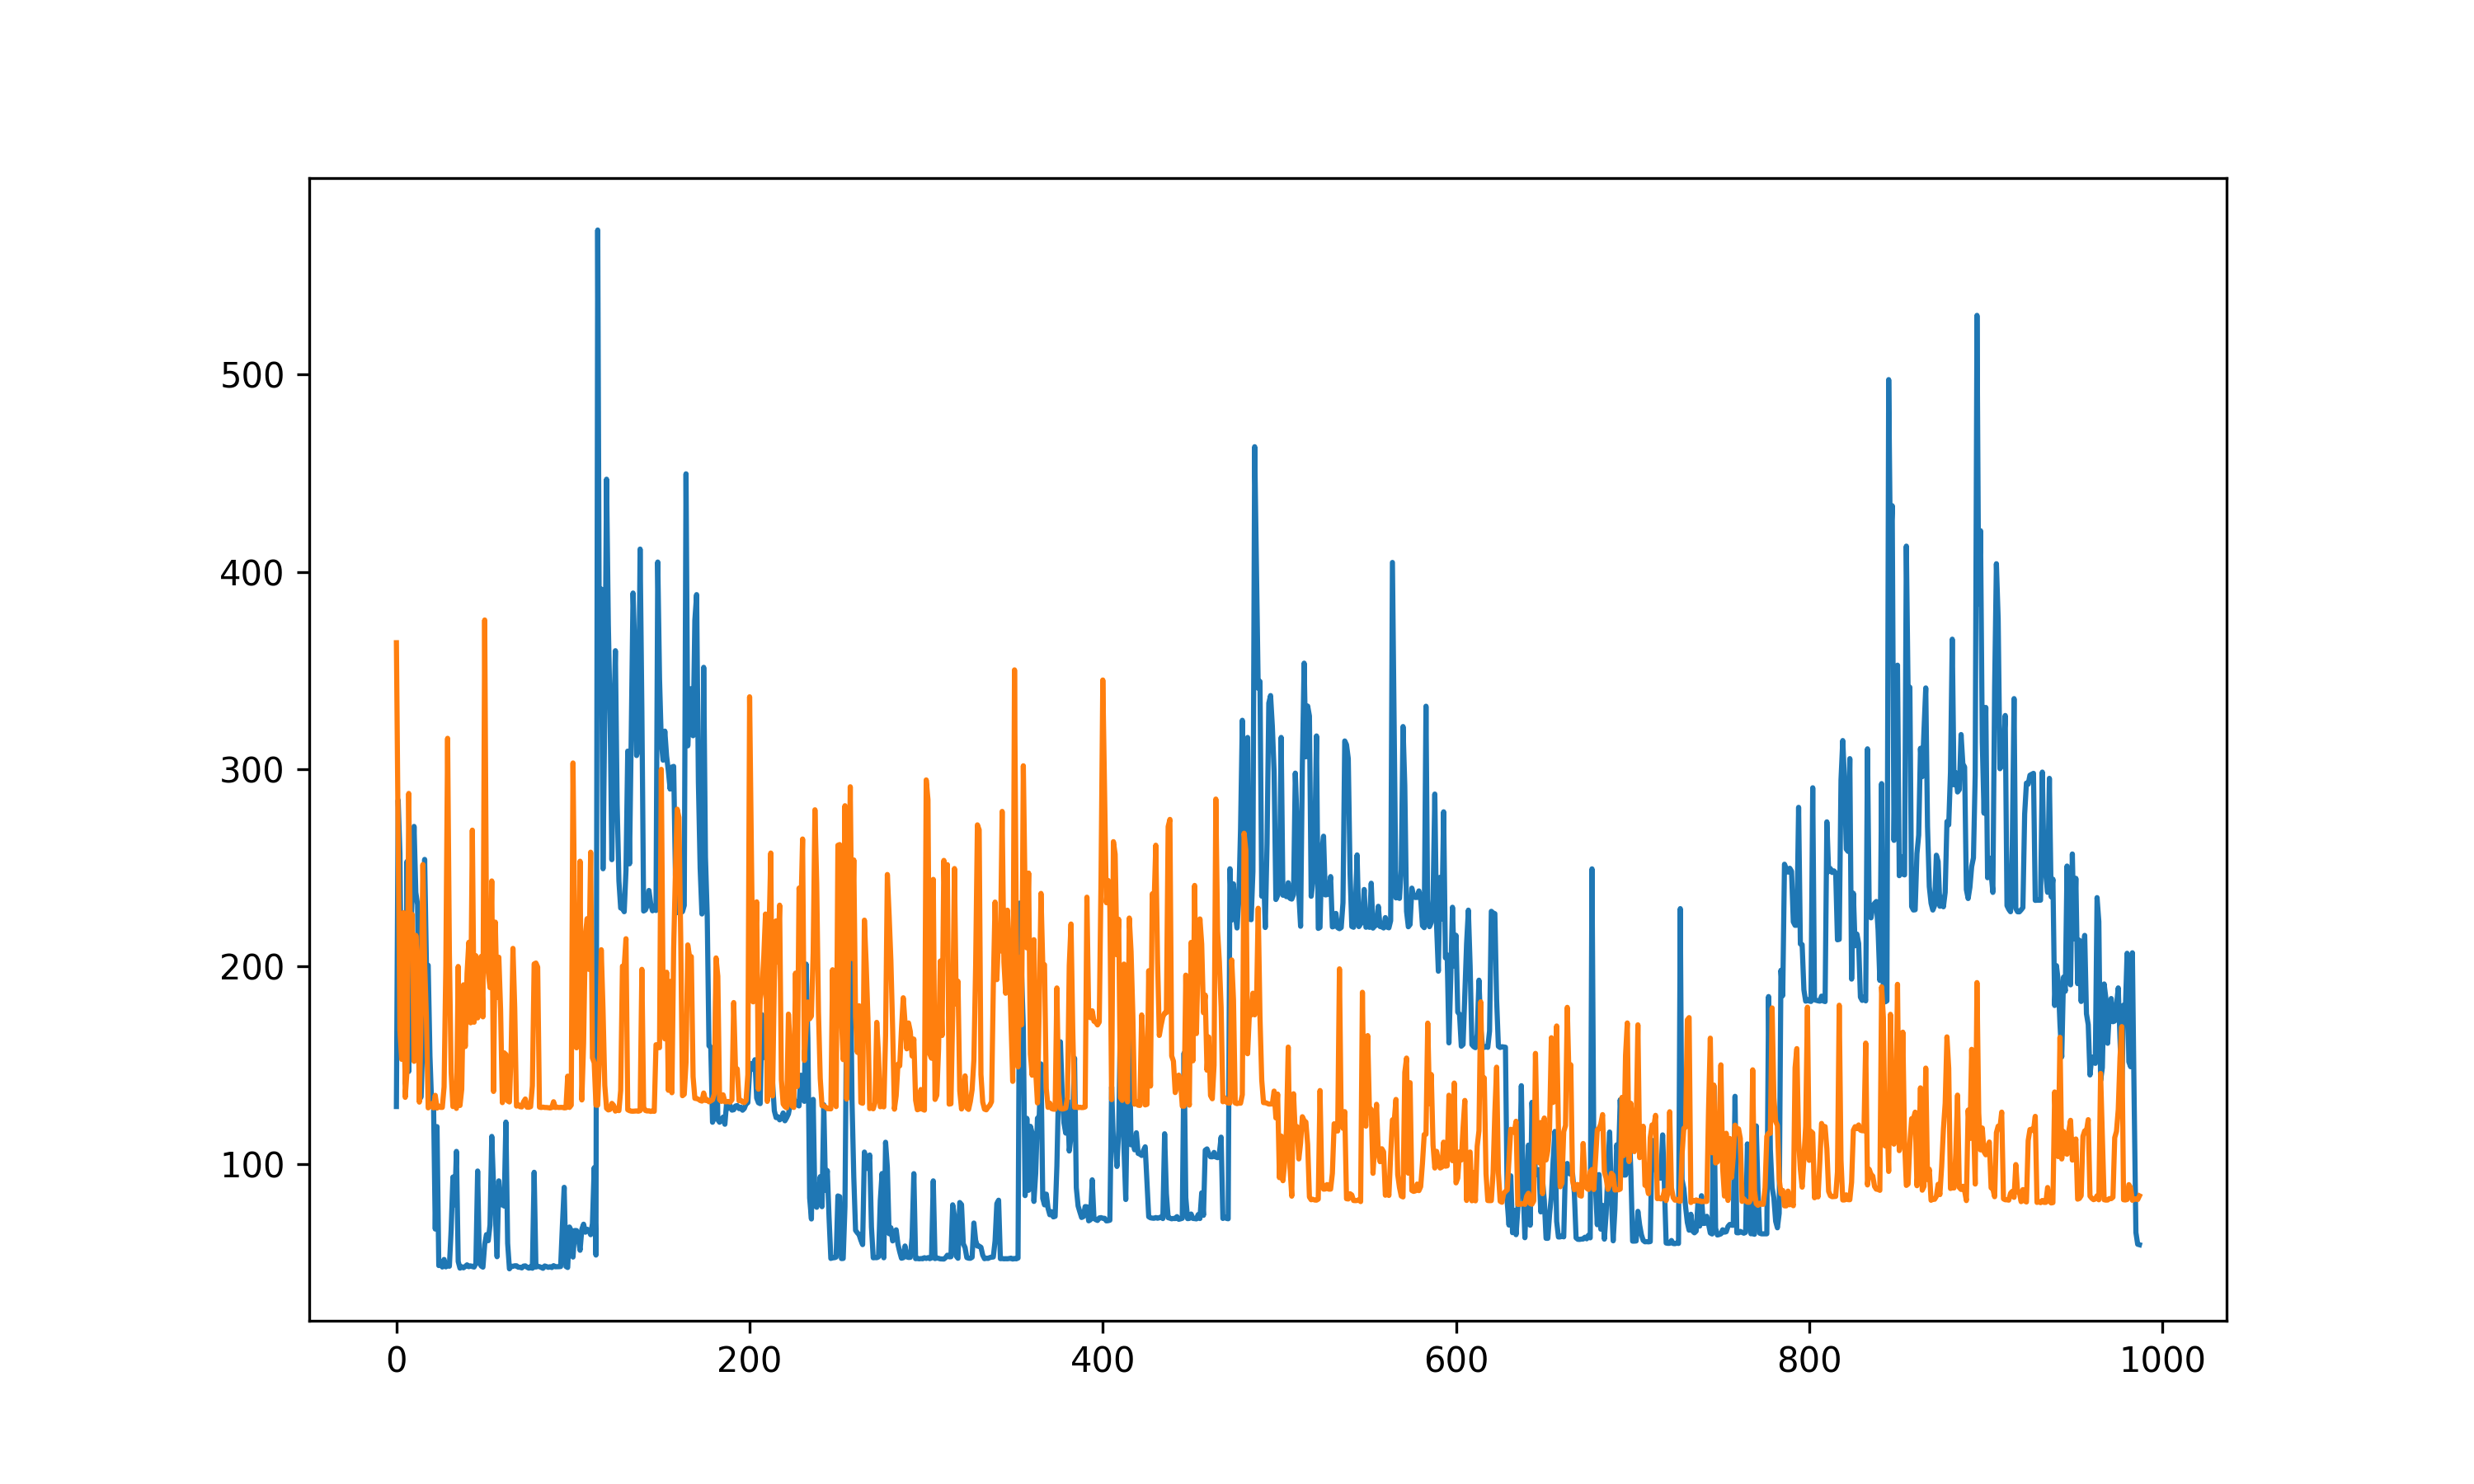
\includegraphics[width=1\textwidth]{plot_0.png}
    \caption{Benchmark 1 and 2 From sleeping Barber}
    \label{fig:bench_1_2}
\end{figure}


\begin{figure}[h!]
    \centering
    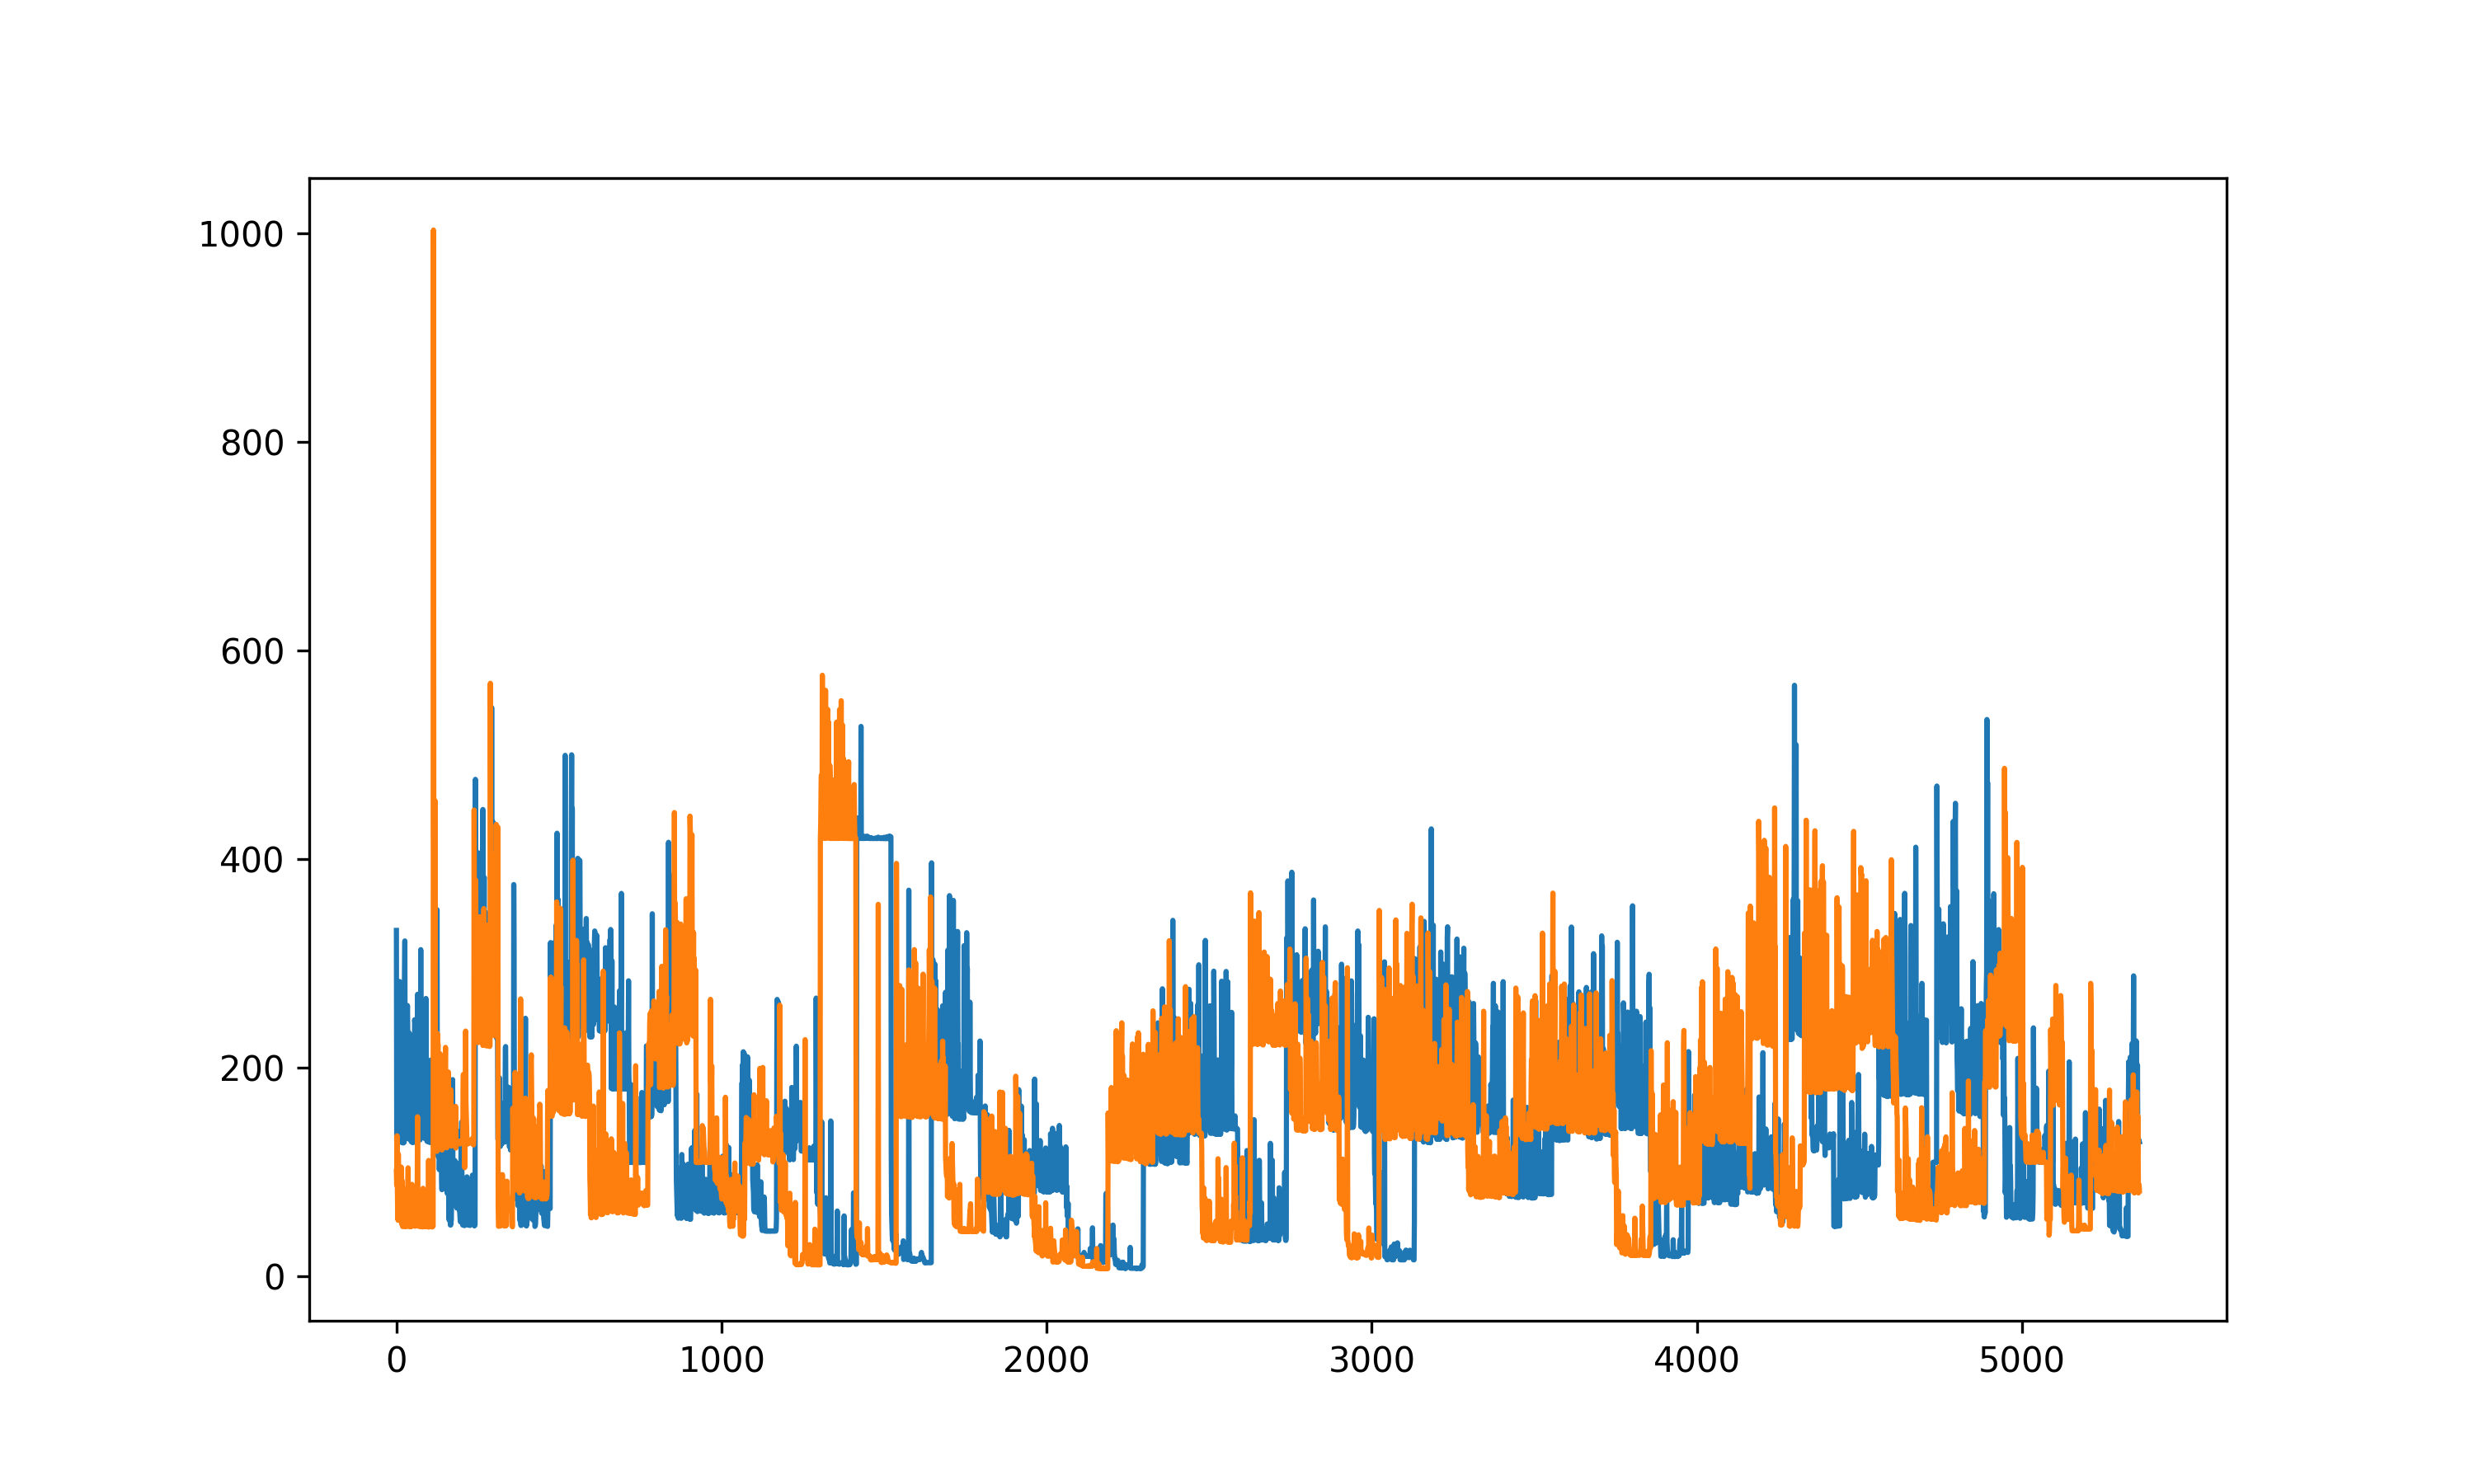
\includegraphics[width=1\textwidth]{plot_1.png}
    \caption{Benchmark 3 and 4 From sleeping Barber}
    \label{fig:bench_2_3}
\end{figure}

\subsection{Presentation of four algorithms to compare curve}

The notion of distance is useful for quantifying and describing the objects present in
a curve, for example. The desire to remain in the space of the image requires the use of specific distances, which provide exclusively integer results. After the definition of use, there is an inventory and a comparison of the main discrete distances used in curve analysis.

\subsubsection{Area method}

First, I have used Area \cite{jekel2019similarity} method to quantify the difference between the curve, this an algorithm for calculating the area between two curves in 2D space.
Strictly speaking, the expression area under the curve refers to the area A of the domain delimited by a curve (represented in an x-y diagram) and three straight lines (the x-axis and two vertical lines with abscissa a and b). If the curve has the equation $y=f(x) y=f(x)$, the area is $A=\int _{a}^{b}f(x)\, {d} x$. This area is a true area (e.g. milliseconds for benchmarks) only if the function f has only positive (or zero) values over the interval [a,b] and if both the abscissa and the ordinate are lengths (with the same choice of unit, e.g. milliseconds for benchmarks).
For the purpose of detecting if the behaviour has changed between two benchmarks, it is not interesting because it quantifies the area a whole and area can be equal but not their behaviour.

\subsubsection{Curve Length Measure}


Let consider in the plane a curve \cite{moran1966measuring} which is the graph of a function f defined on the interval [a, b]. For example, the algorithm will calculate the length of this curve. To do this, we will approximate the curve by a broken line formed of n segments and calculate the distance of this fractured line. We will then obtain the exact length of the curve by a limit process.
Theoretically, the length of the curve representative of a function f over an interval [a; b] (on which it is differentiable) is given by $\int_{a}^{b} \sqrt{1+f^{\prime}(x)^{2}} d x$
This makes it possible to obtain the exact value compared to the initial problem as well as an approximate value and appreciate the accuracy of the algorithm according to the value of n. So we are sure that the value is an exact value and not an approximation compared from the Area method, for example.

The curve length measure could work to differentiate the algorithm that has a lot of variance difference across the benchmark. This is not always the case because sometimes both benchmarks can I have a kind of flat curve, or can I have no steady state.
The application of the curve length measure used in this dissertation is from \cite{jekel2019similarity}
\subsubsection{Hausdorff Distance }
The Hausdorff distance \cite{belogay1997calculating} is used to account for the maximum deviation between two polylines (benchmarks 1, benchmarks 1). By definition, two polylines benchmarks one and benchmarks 2 are at a Hausdorff distance (DH) from each other of less than d units, if each point of L1 is within d units of at least one point of benchmarks 2, and if, reciprocally, each point of benchmarks 2 is less than d units away from each other by at least one point of benchmarks 1.

The Hausdorff distance is defined as the greater of the two following components :

\begin{itemize}
    \item The first distance which is the largest value of the non-symmetrical distance from benchmarks 1 to benchmarks 2,
    \item The second distance which is the largest value of the non-symmetrical distance from benchmarks 2 to benchmarks 1.
\end{itemize}


For this project I'm using the implementation of the library scipy which is implemented and documented here \url{https://docs.scipy.org/doc/scipy/reference/generated/scipy.spatial.distance.directed_hausdorff.html}

From this principle and from the scipy documentation, we are taking the two distance produced by the algorithm then taking the minimum to avoid false positive.

This distance has the advantage of providing two measurements. Right-of-way lines can thus be compared using the component starting from the shortest line. On the other hand, the Hausdorff distance, with the disadvantage of calculating the
distance on the nearest pairs of points and not on homologous points. Homologous points are points that visually correspond to each other. For example, the point in benchmark 2 used to calculate distance one is not the Intuitively corresponding to the point of benchmark 2; it is simply the closest point. The distance from Hausdorff considers polylines as simple sets of dots unordered. This problem is particularly important for very sinuous or with loops. Small distances can then be sent back to different lines. Similarly, pairs of dots cannot be considered to be matches. Nevertheless, this particularity has the advantage of reducing calculation time: the algorithmic complexity of this algorithm is linear. 


This method seems to be working better because there is no need for the dataset to know if the first measurement of the first sequence must match the first measurement of the other sequence and that the last measurement of the first sequence must match the last measurement of the other sequence (but it must not be its only match).


\subsubsection{DTW}

 The DTW finds the best match between a reference (the score) and a signal (the interpretation) by calculating a difference between vectors of the characteristics for each of these signals. The comparison algorithms of changes are based on the exact correspondence between the reference and the signal and do not take into account, among other things, the imprecision of the pitch estimation due to chords or errors of the height detection algorithm. In addition, the DTW can be used to align continuous multi-dimensional characteristics, for example, results from a signal analysis, which allows the partition alignment to be based on parameters such as the number of partitions, the size of the partition, the number of partitions, the number of partitions to be aligned, the number of partitions to be aligned, the number of partitions to be aligned, the number of partitions to be aligned and the number of partitions to be aligned.
The system does not require prior segmentation of the benchmark measurements and does not require prior segmentation of the
signal.
In short, the DTW algorithm consists of three steps:

\begin{itemize}
    \item Calculation of local distances
    \item Dynamic programming to obtain the global optimum \begin{itemize}
        \item a) Calculation of increased distances. Only the minimum predecessors are kept. of each point => local optimum
        \item b) Backtrack to find the minimum distance => global optimum
    \end{itemize}
    \item Result: A shift path that consists of the correspondence of the two equations.
\end{itemize}

The effectiveness of DTW was not worth because sometimes for very long benchmarks the algorithm needed a lot of memories in fact, I could not run it in my computer for 5000 measurements because it took more than 8 gigabytes.
Also from the results, it needed data preparation to be run correctly by with no good result as the Hausdorff distance \ref{result}

The application used in this dissertation is a work done by \cite{salvador2007toward}

\subsection{ interpretation of results after running the algorithms}

After Choosing the two benchmarks, I ran each algorithm on each experiment of the barber problem.
The one \& two experiments are not similar in contrary to the 3 \& 4, which are similar by human eyes.
Each output of each algorithm is put inside this tabular.


The first result is the area difference between the two curves (more significant number mean bigger area difference).

The second result is the total length difference of the two curves (more significant number mean bigger length difference).

The third result is the cost which is the sum of absolute differences, for each matched pair of indices, between their values.

The last result is the sum of each pair of the distance subsets are from each other which seems to work the best from my experiment because of the low score difference that has been given for the by the eye the same benchmarks.

\begin{table}[h!]
\begin{tabular}{|l|c|c|c|c|c|c|}
   \hline
   benchmarks  & area & curve length & DTW & directed Hausdorff \\
   \hline
   1 \&  2 & 313 & 81918 & 14 & 68757 & 197\\
   \hline
   3 \& 4  & 295 & 32960 & 48 & 191649 & 7 \\
   \hline
\end{tabular} \\ 
\caption{Comparaison between two inequal benchmarks and two equal benchmarks}
\label{result}
\end{table}


As expected, the only algorithm that seems to work is the directed Hausdorff algorithm because it is not influenced by the size of the dataset, indeed as the curve length increase the difference of the score increase. 
I order to classify if a benchmark has changed between 2 commits, I have to found a threshold where, if the result of an algorithm would surpass this threshold it will mean that the benchmarks have changed from the previous commit. I order to get that threshold I labelled by hand all the benchmarks by hand. For 50 benchmarks by hand six have a real changed by human eyes and the rest have not changed between commit. Those 50 benchmarks could be corresponding to our training data. The threshold that seems to better classify is 20 because based on that, the result of the directed Hausdorff algorithm is that value that is better to separate the behaviour changed benchmarks and those who have not changed.
I have put a threshold of 20 with the directed Hausdorff. When the directed Hausdorff value is more than 20 is interesting to look at the benchmark because it means that there is a significant difference between the two benchmarks.


\subsection{Usage for different example}


In order to prove the usability of the usage of the Hausdorff distance, I decided to run a few more tests on other benchmarks.

For that, there is a script inside the corpus of this dissertation which is called compare.py it takes two commits (iteration of the code) as parameters and then retrieves all the data from those benchmarks then run the comparison and tell if the benchmarks result have performance difference. \\

\begin{figure}[]
    \centering
    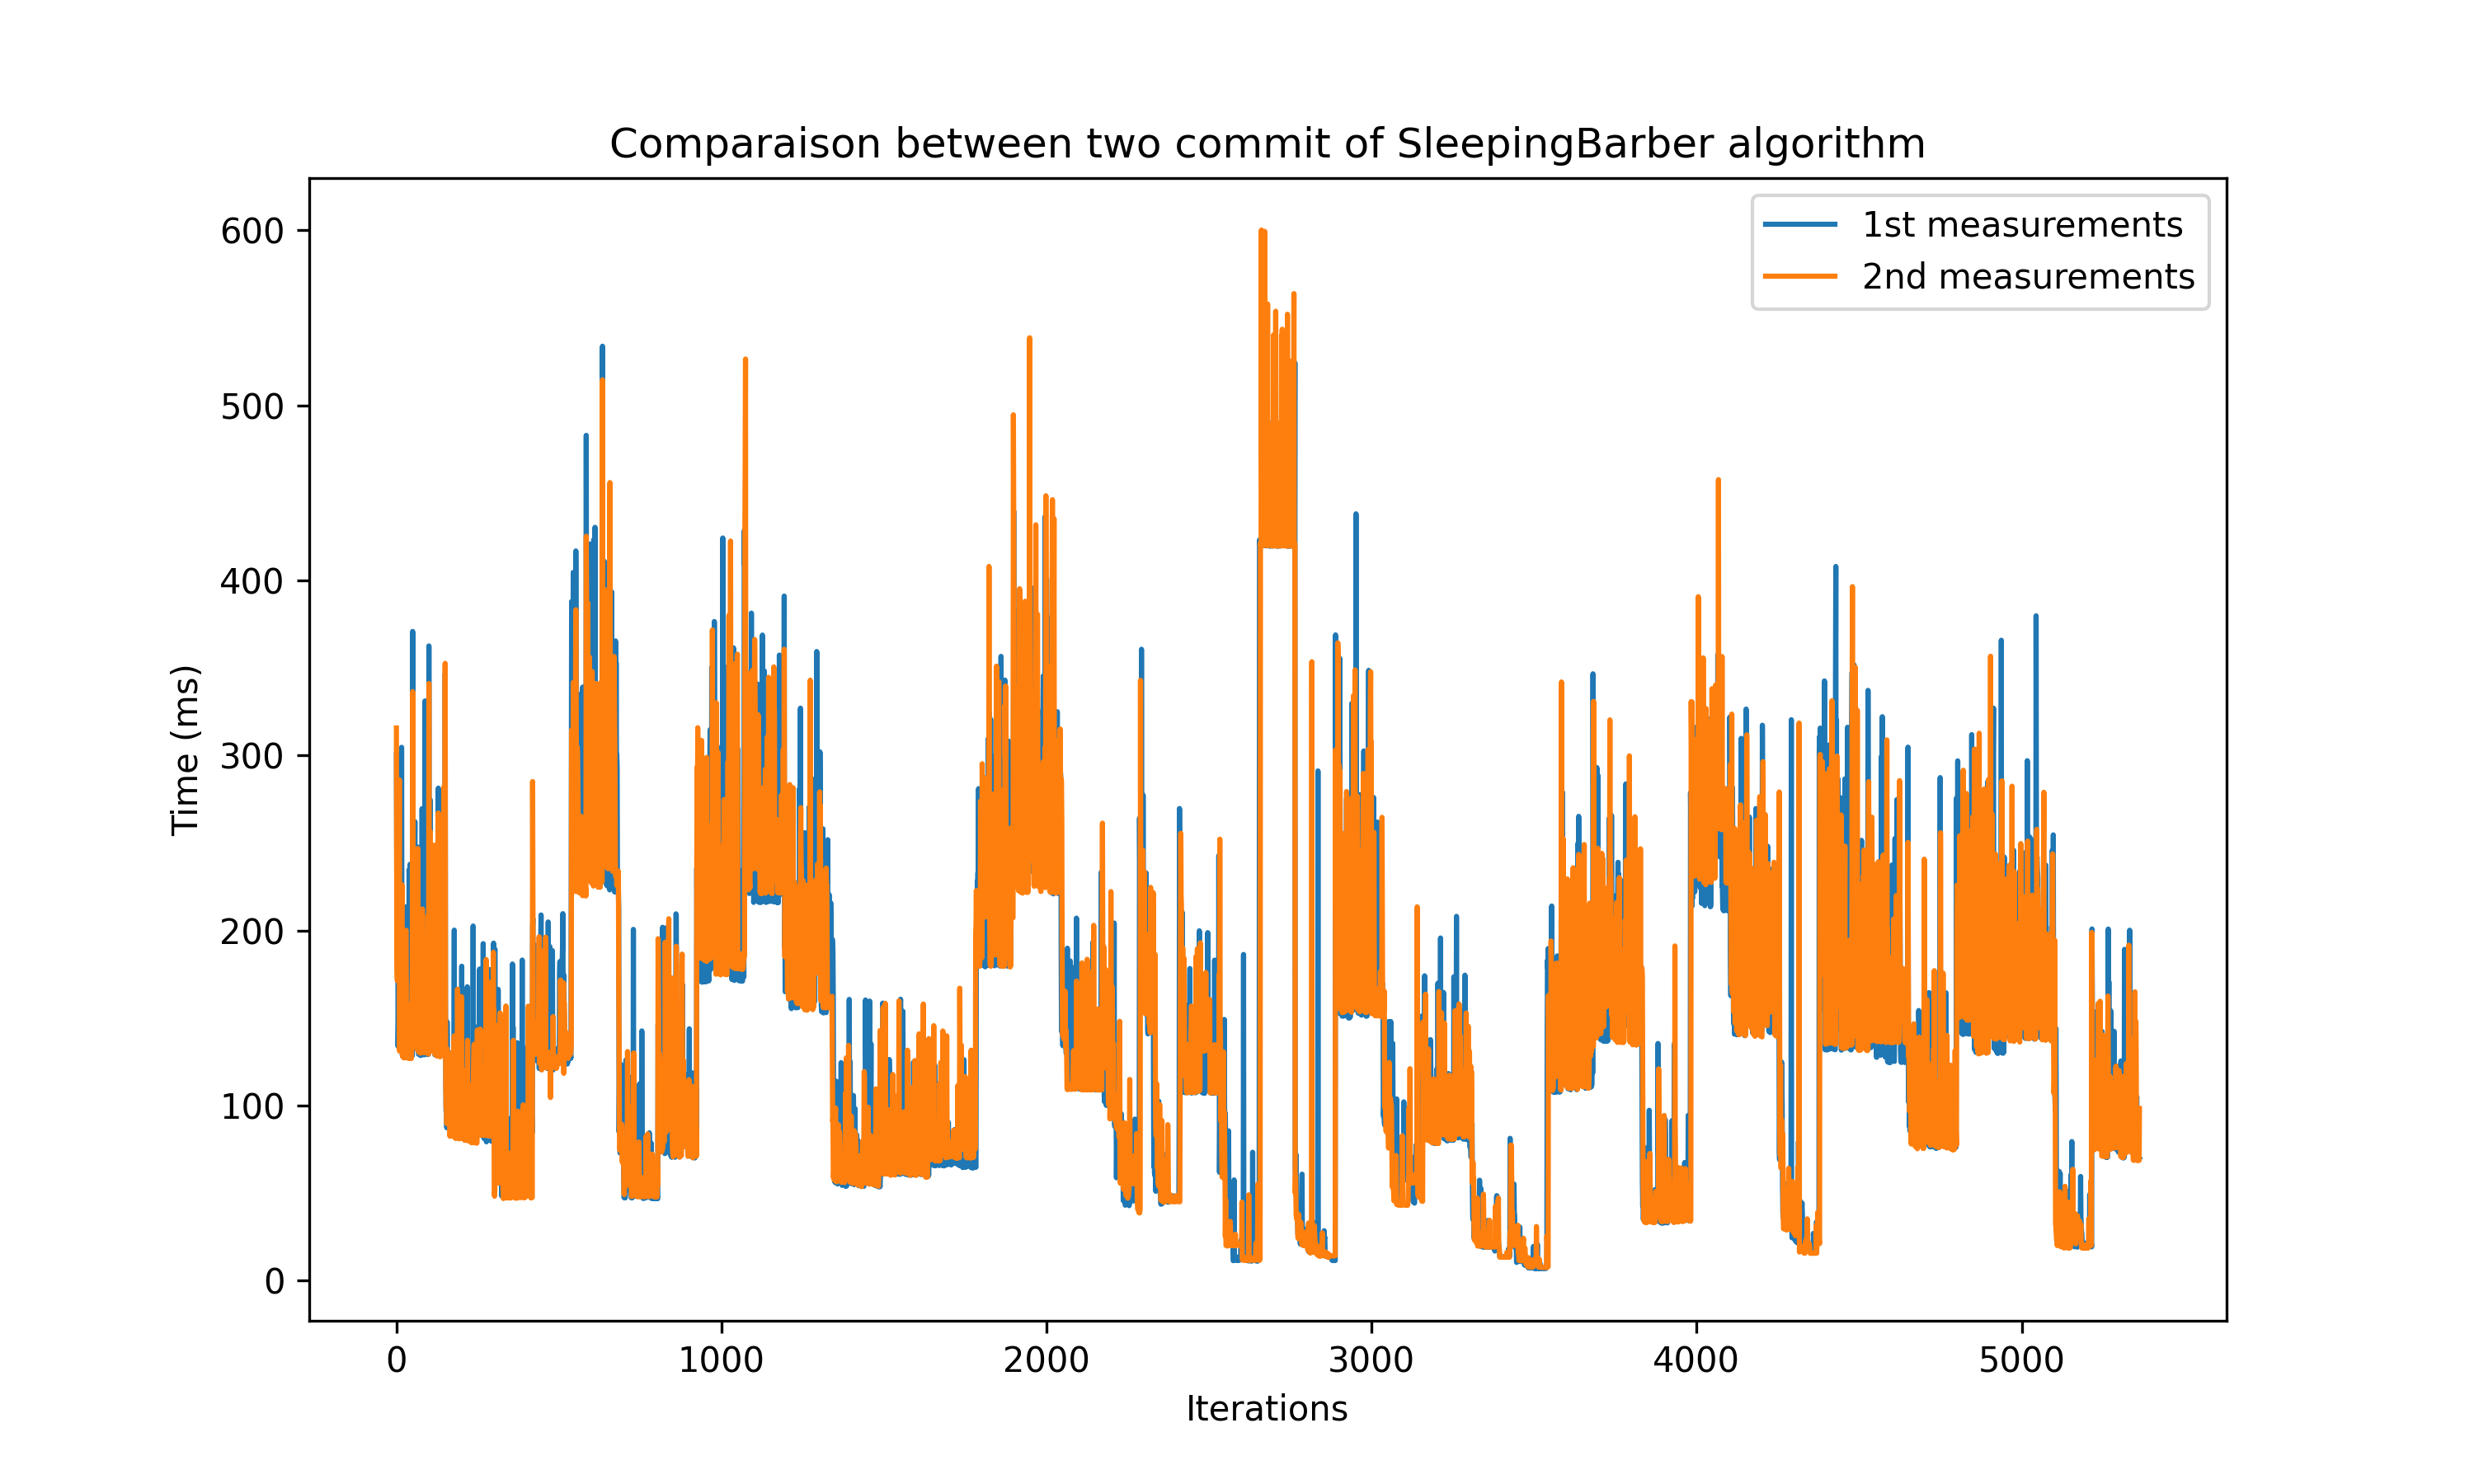
\includegraphics[width=1\textwidth]{images/plot_SleepingBarber_4.069999999999936.png}
    \caption{Benchmark 1 and 2 from sleeping Barber which are classified as having the same performance difference}
    \label{fig:bench_1_2_1}
\end{figure}

\begin{figure}[]
    \centering
    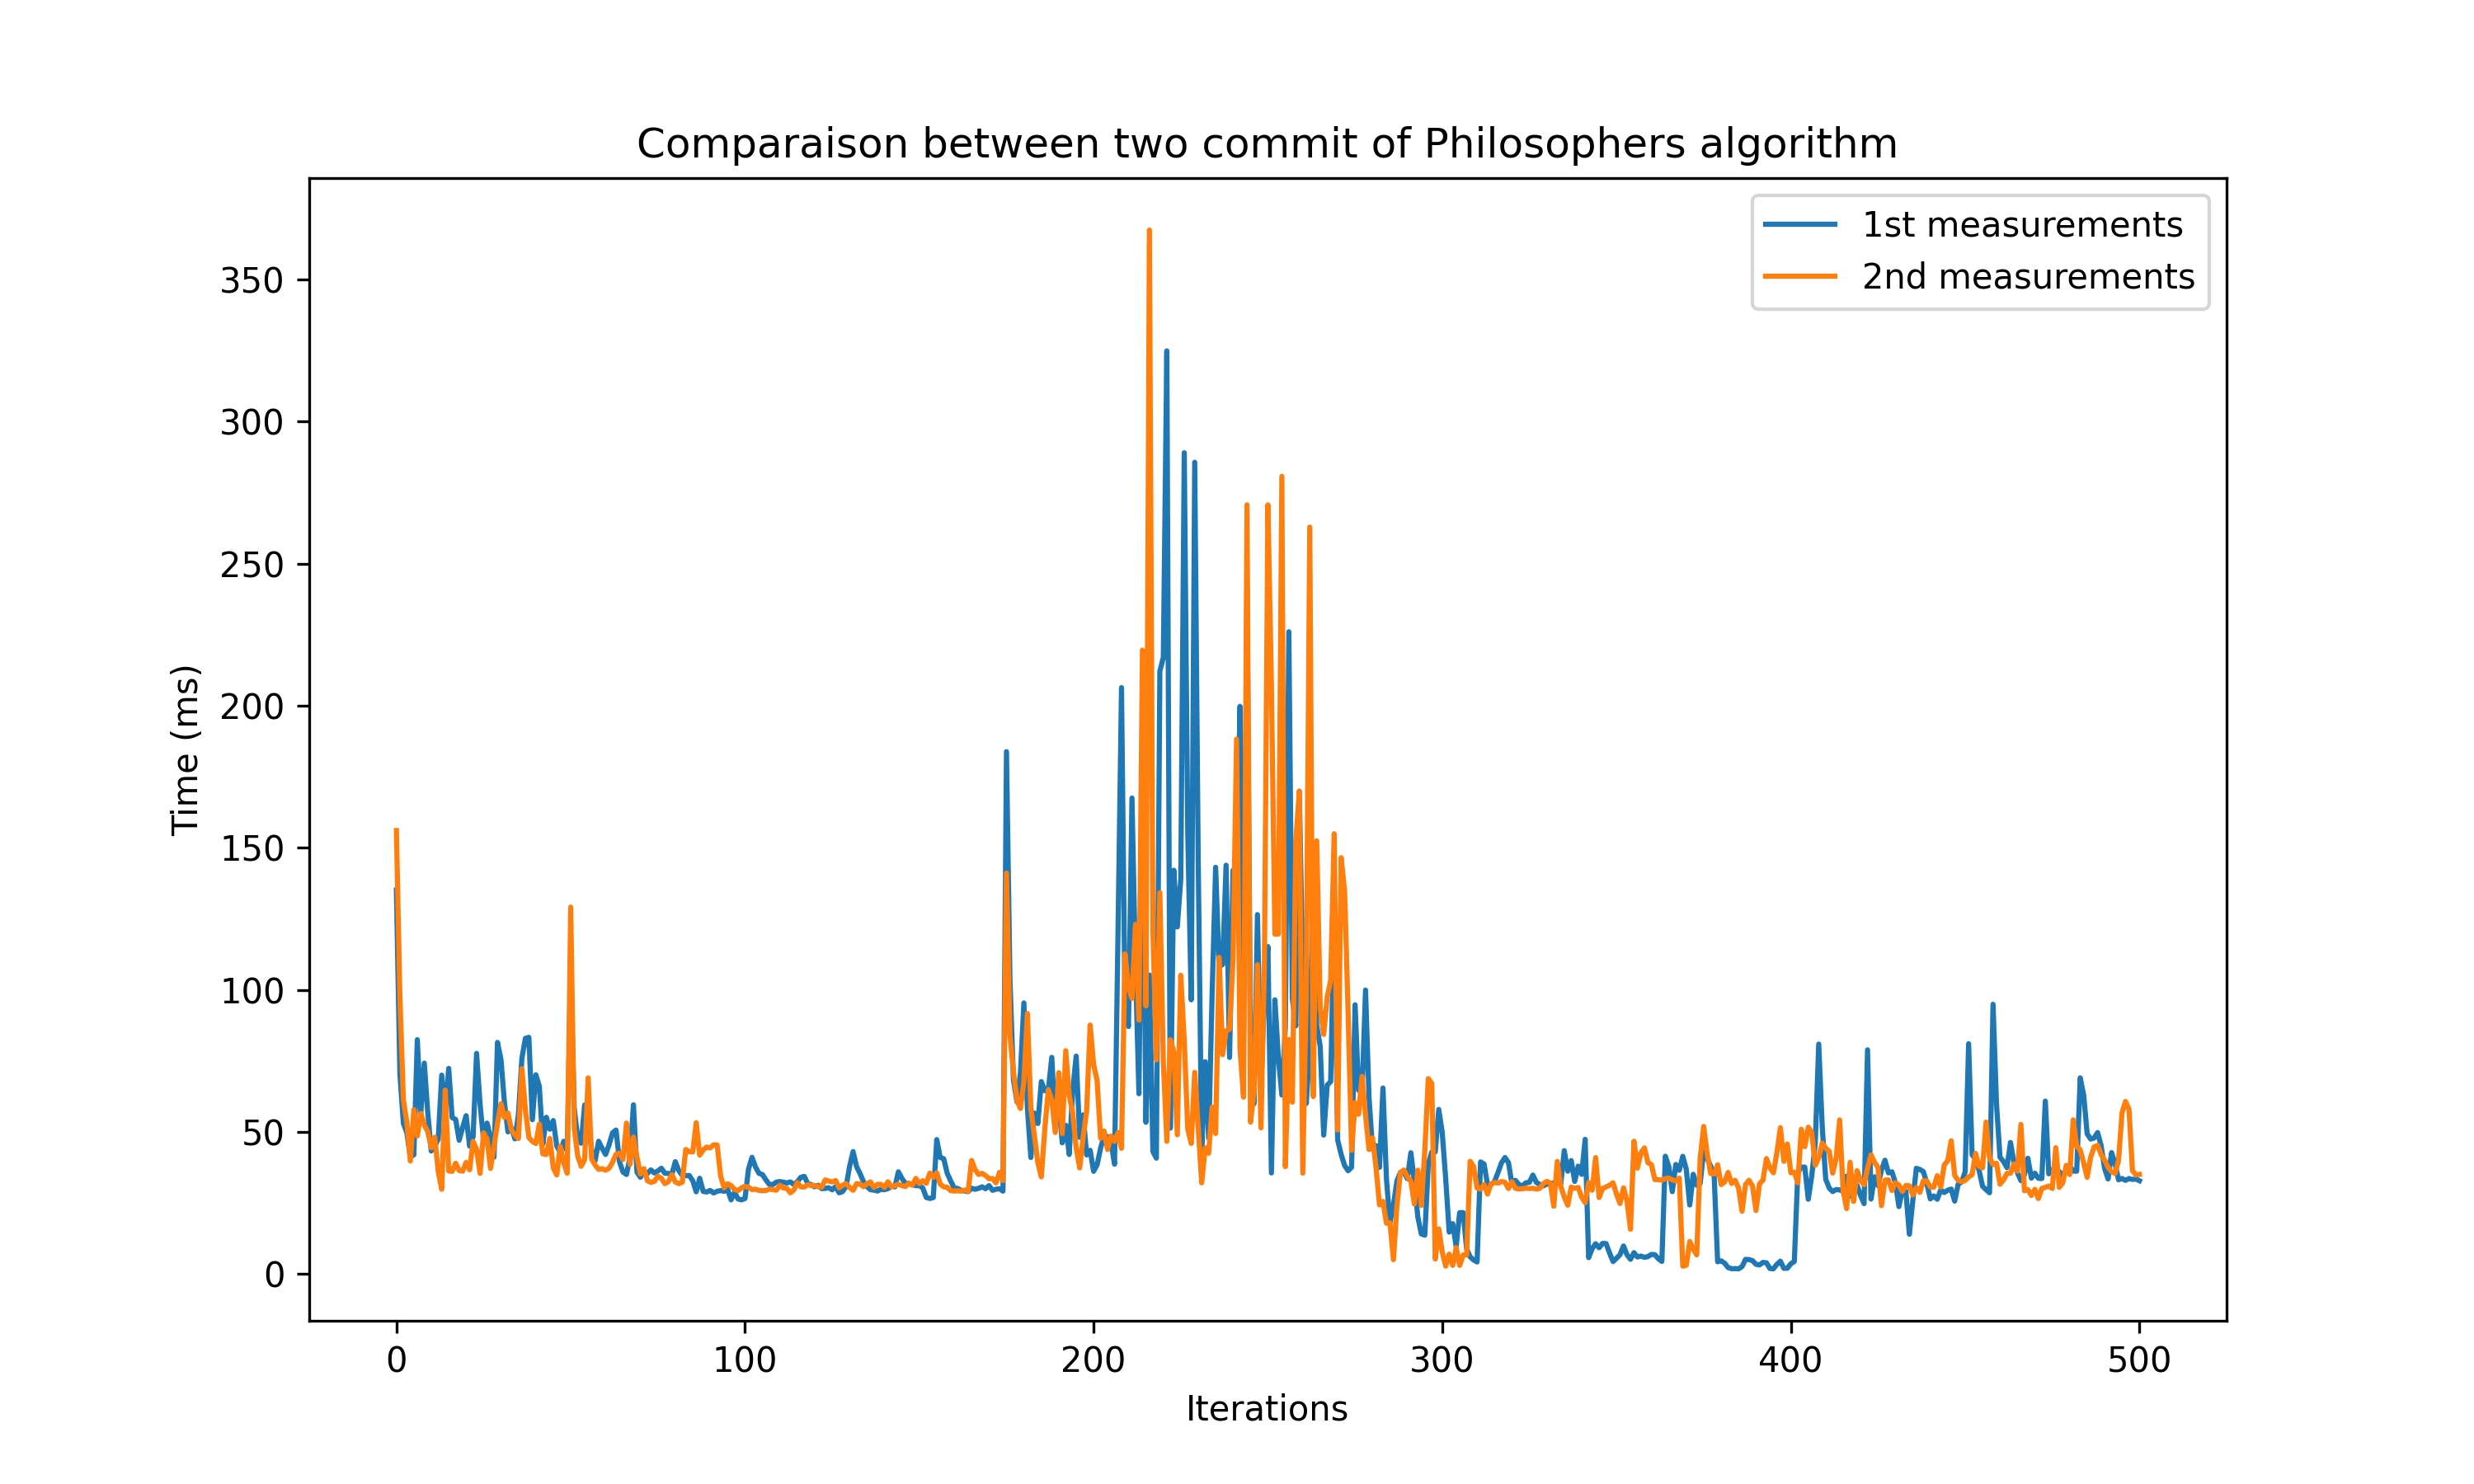
\includegraphics[width=1\textwidth]{images/plot_Philosophers_42.533000000000015.png}
    \caption{Benchmark 1 and 2 from Philosopers algorithm which are classified as not having the same performance}
    \label{fig:bench_1_2_2}
\end{figure}

\begin{figure}[]
    \centering
    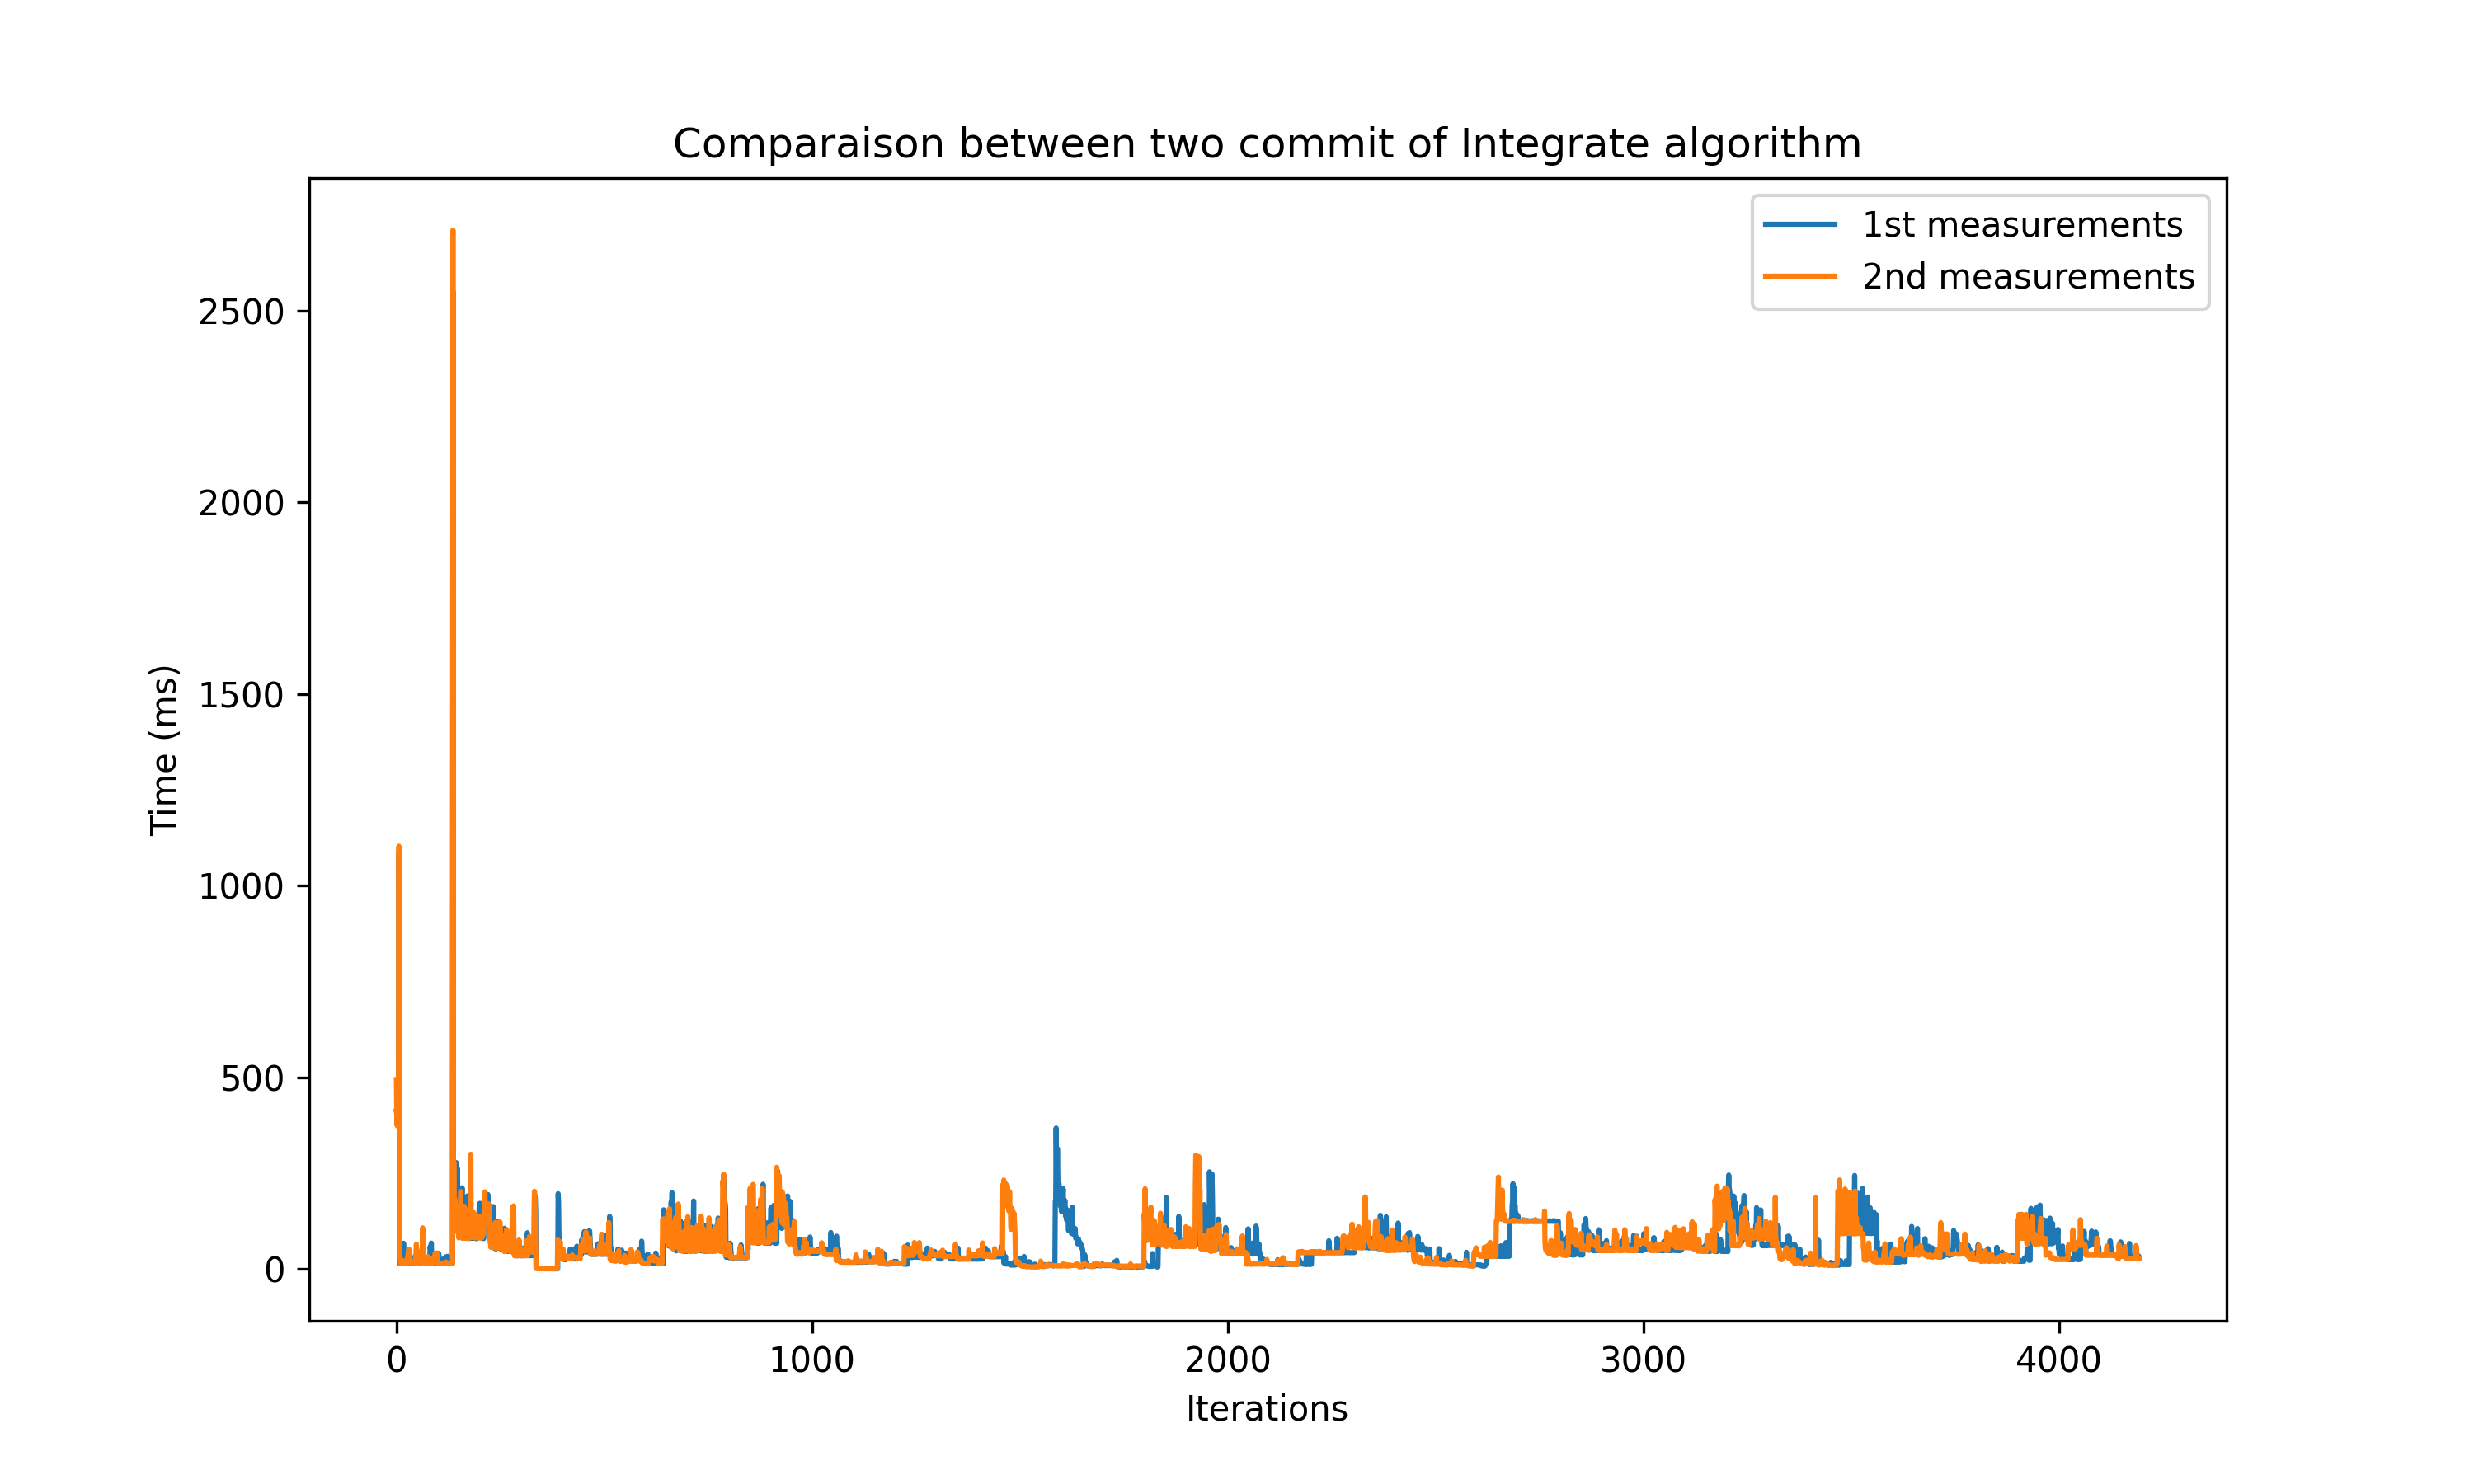
\includegraphics[width=1\textwidth]{images/plot_Integrate_159.78600000000006.png}
    \caption{Benchmark 1 and 2 from Integrate algorithm which are classified as not having the same performance}
    \label{fig:bench_1_2_3}
\end{figure}


\begin{figure}[]
    \centering
    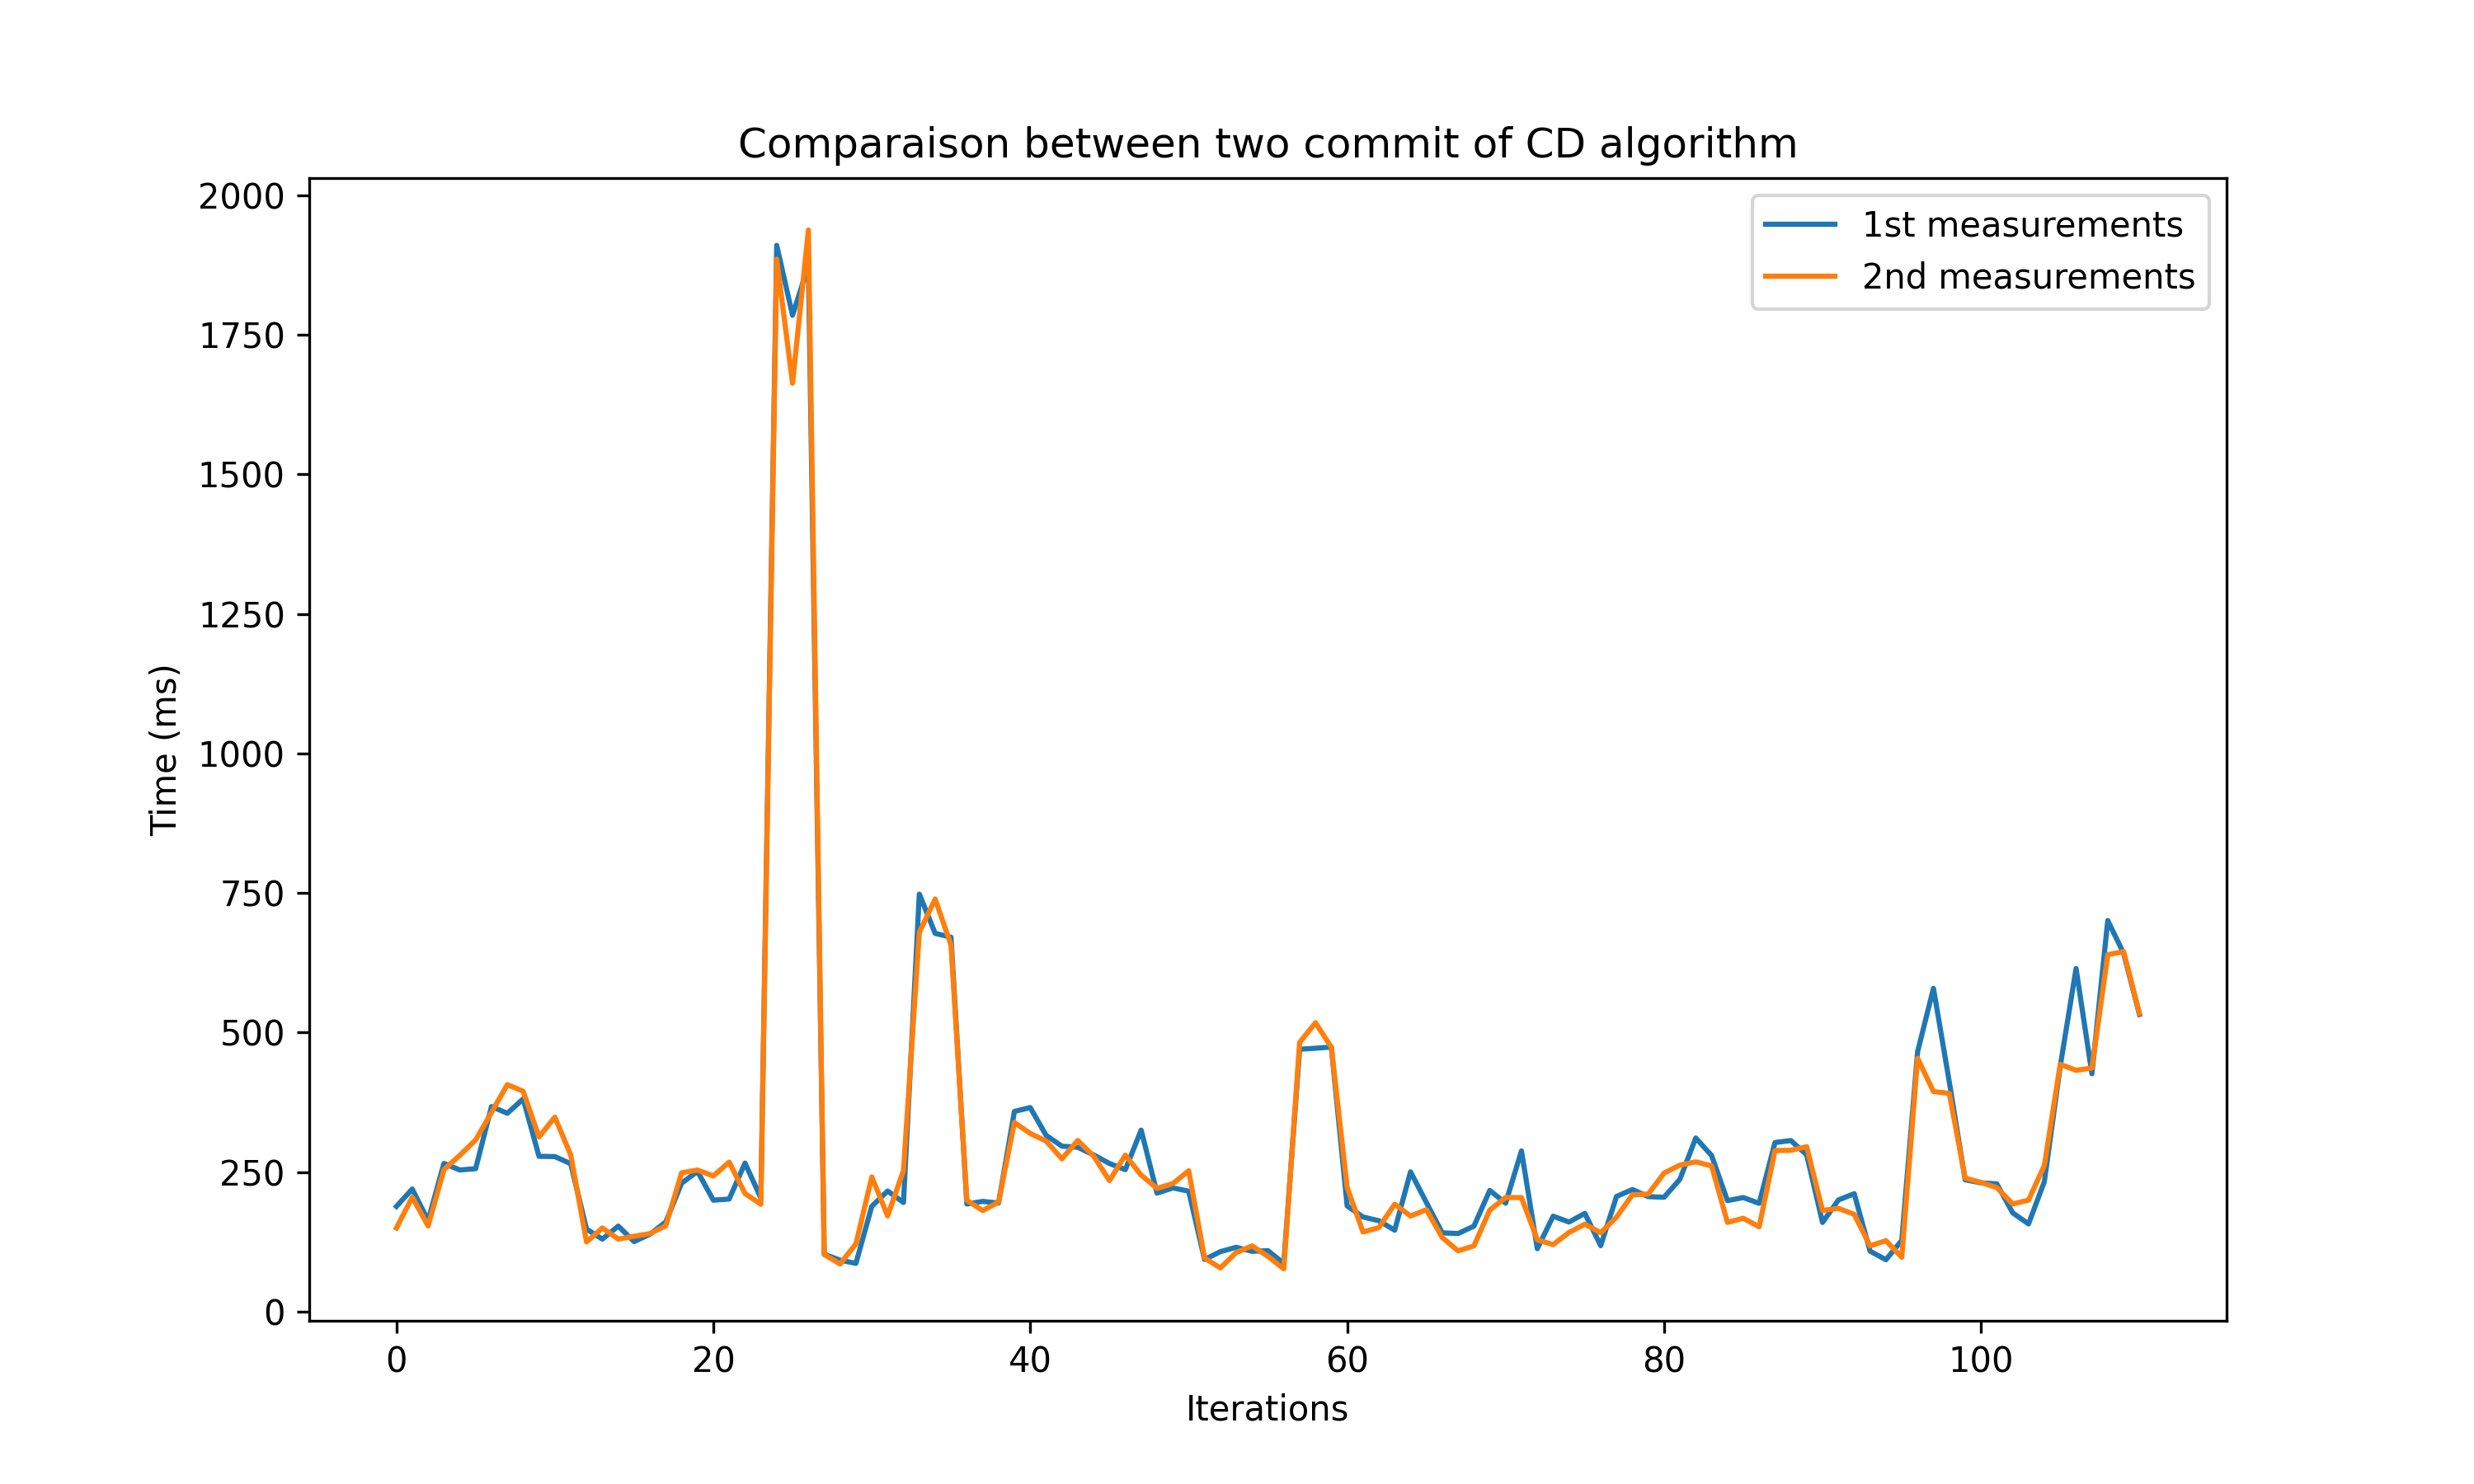
\includegraphics[width=1\textwidth]{images/plot_CD_100.56999999999994.png}
    \caption{Benchmark 1 and 2 from CD algorithm which are classified as not having the same performance}
    \label{fig:bench_1_2_3}
\end{figure}


\begin{figure}[]
    \centering
    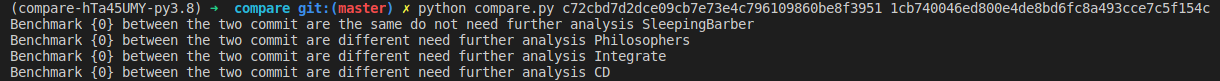
\includegraphics[width=1\textwidth]{images/Screenshot_20200829_135418.png}
    \caption{Screen shot of the script giving the result of the classification}
    \label{fig:bench_1_2_4}
\end{figure}

As you have seen the result for from figure \ref{fig:bench_1_2_3} could be classified as the same by human eyes but it depends on where do you put the threshold the result from this comparison with Hausdorff distance was "50.24" which is above the threshold given in the script a big threshold should mean less sensitivity for the performance difference detection.\\

\pagebreak
\newpage


\subsection{Conclusion of classification of variation of behaviour between benchmarks}

The validation of an unsupervised classification, as well as the choice of the number of the group always remain open questions. On real data, recognized criteria such as the distance difference or the silhouette index are optimal with only two groups, limiting the contribution of such an analysis.
Future work might be to automatically find the threshold without labelling the data by hand and finding the best threshold for the quantify algorithm.
I could be interesting to apply the directed Hausdorff to more use case than the sleeping barber experiment in the future.
This method works well, but as you have seen, it is not automatic you need to put manually a kind of threshold which is not suitable.
A future approach would be to learn for those thresholds and maybe determine an optimum threshold from a kind of algorithm.



\section{Setup Of Rebench Data}
This section will talk about more about the engineering process for rebench data and how it could be deployed and used in the future.\\

\subsection{Building a REST API around the database structure}

First thing I did was take the data collected, which is produced by rebench \cite{ReBench:2018}. The data is in Postgres SQL format, which is a language for communicating with a database. This computer language is notably very much used by web developers to describe with the data of a web site (Here a REST API).

To import the backup of the data produced by Rebench I am using this command which will import only the data and not the structure which is created by the node.js server.

\begin{python}[h!]
pg_dump --verbose -Fc -U postgres -h 0.0.0.0 -p 5432  -a --dbname=postgres > data.dump
\end{python}

The structure was designed by \cite{ReBench:2018}, but I include a map of the structure to see it more clearly.


\begin{figure}[h!]
    \centering
    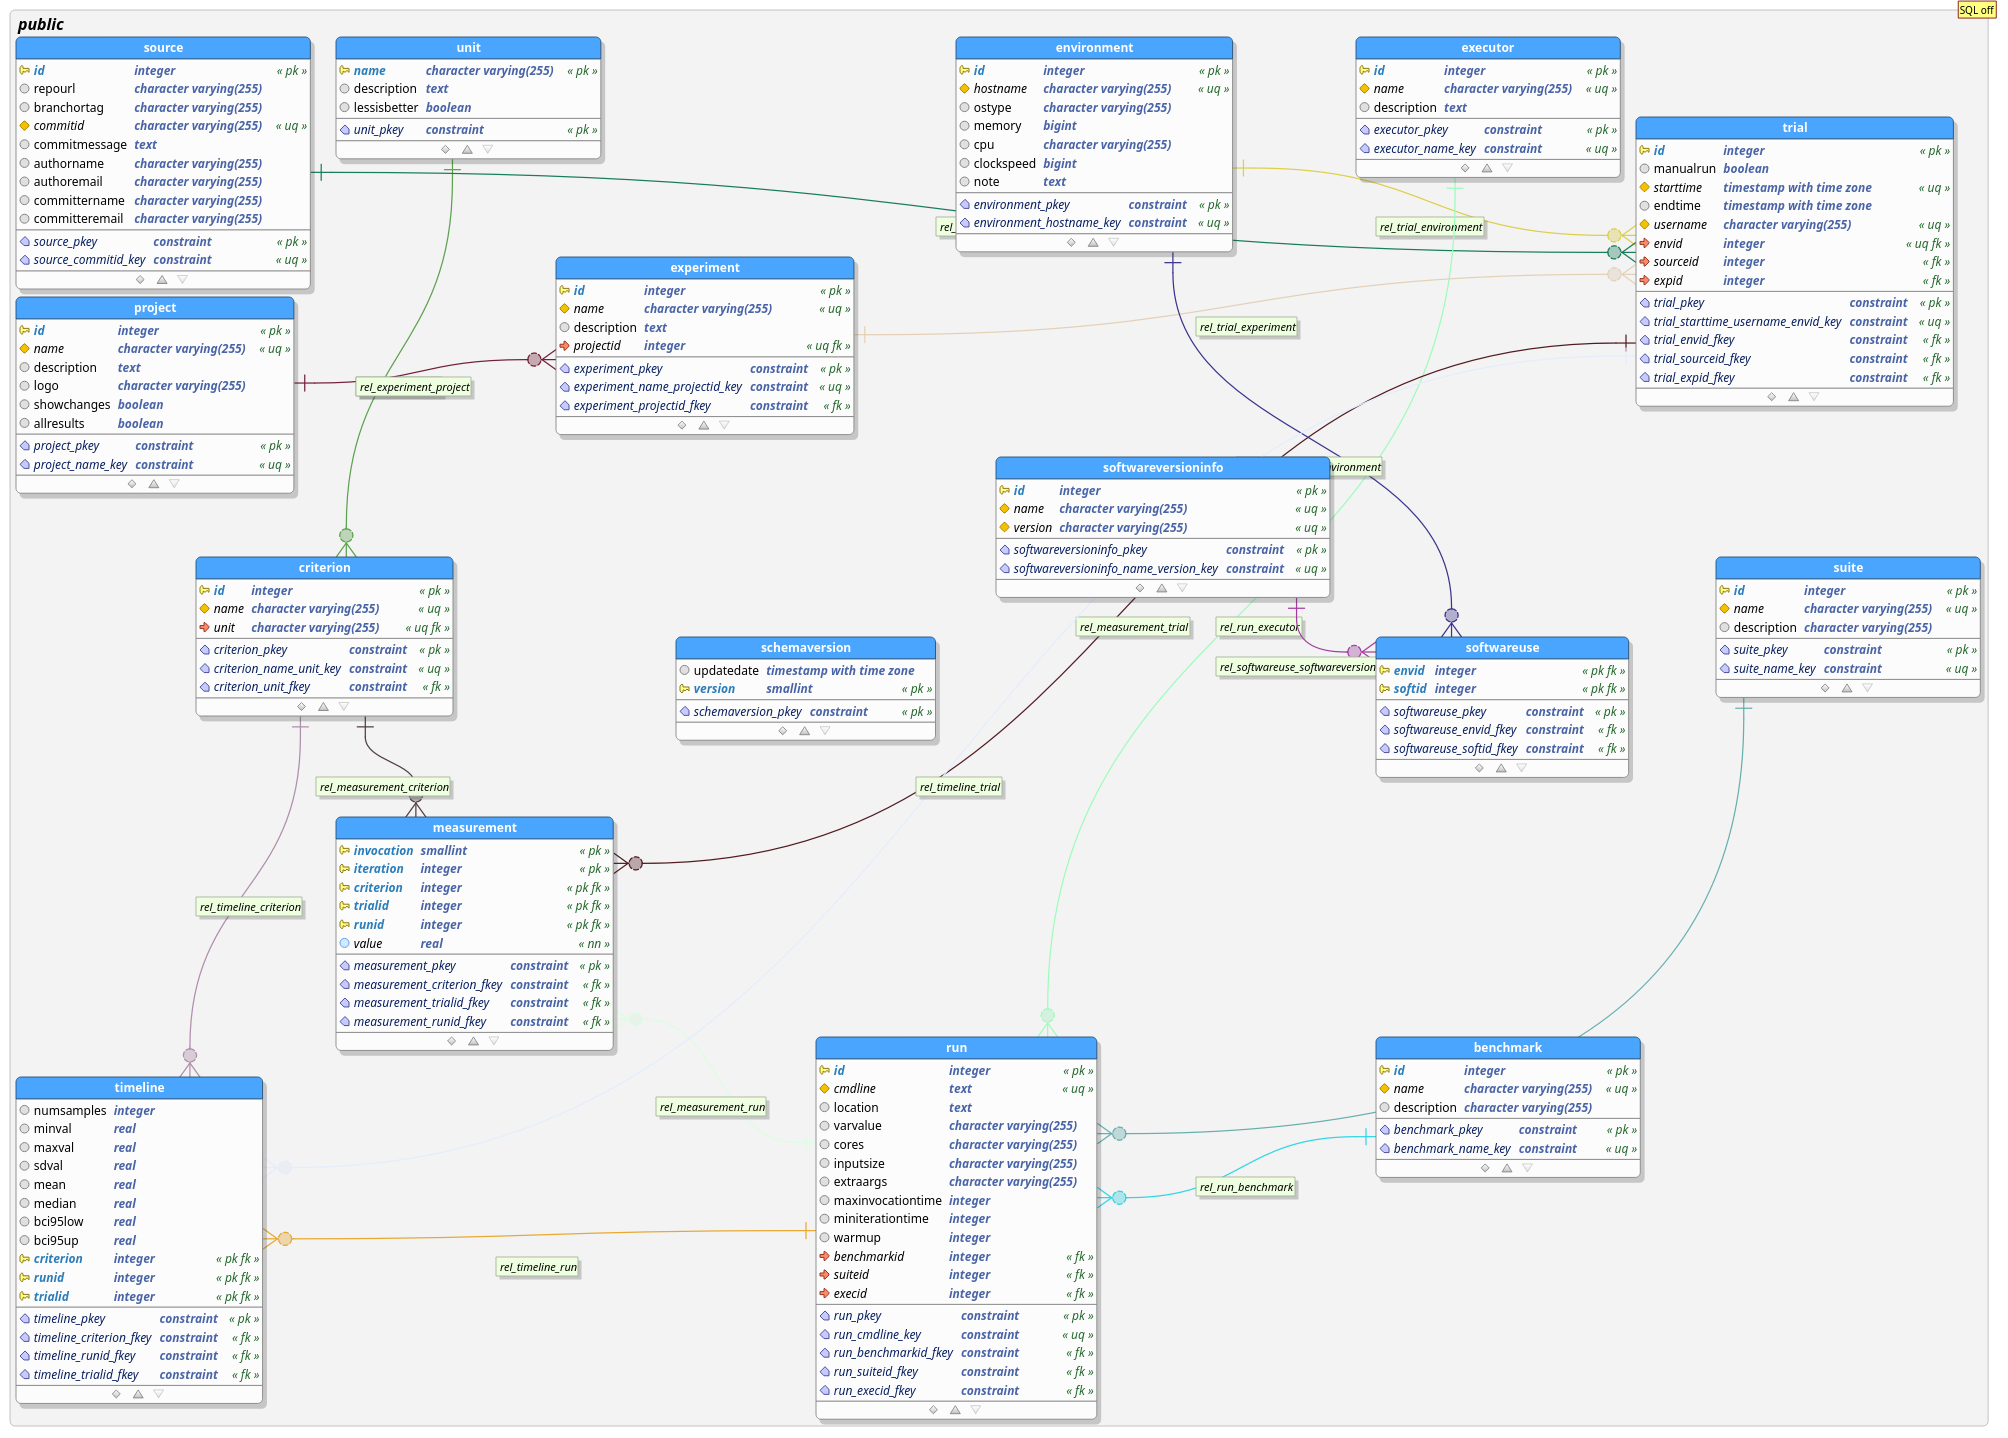
\includegraphics[width=1\textwidth]{images/database.png}
    \caption{Database Structure}
    \label{fig:database}
\end{figure}

The database is run in a docker container. I will explain it later.

After that, I needed to manipulate them, so I build a REST API which is a style of architecture for building applications. It is a set of conventions and best practices to be respected and not a technology in its own right. The RESTful architecture uses the original HTTP protocol specifications, rather than reinventing an overlay.

\begin{itemize}
    \item The URI as a resource identifier
    \item Using HTTP verbs as operation identifiers (GET, POST, PUT...)
    \item HTTP responses as resource representation
    \item Links as a relationship between resources
\end{itemize}

Because of the data is created by rebench is from a PostgreSQL database the goal is to add a PostgreSQL connection so that we can retrieve information from a database and display that information in the application as a simple list.
We will use PostgresqlQL as the database. For this, we will use an ORM (Object Relational Mapping). There are several ORM node.js such as Sequelize, type ORM and mongoose. The most suitable ORM in our case is sequelize. Sequelize allows the use of a database type: MySQL, Postgres, SQLite and Microsoft SQL Server but for this project, we will stick to Postgresql.

To communicate with the database, I'm using an ORM (Sequelize) between the database language SQL and the javascript side \cite{pereira2016working}. ORM or Object Relation Mapping is a mapping process between objects and relational database systems. An ORM (here Sequelize) acts as an interface between two systems (Postgresql and The node.js Server). ORMs offer to the developers' basic benefits, such as reducing time and effort and focusing on business logic. The code is robust instead of redundant. ORM helps manage queries across multiple tables efficiently. Finally, an ORM (such as Sequelize) is able to connect to different databases (which is useful when switching from one database to another).



To Serialize the data I'm using TSOA, which is a framework to build REST.API in typescript it builds around express.js, node.js and typescript

For this project, I am only implementing the GET method for the route that need an id as the GET parameter. This means we should have a URL like this: /benchmarks/1. It's easy to do when you are building the road.

This is the implementation.

\begin{python}
...

export interface IBenchmark {
  id: number;
  name?: string;
  description?: string;
  logo?: string;
  showchanges?: boolean;
  allresults?: boolean;
}

@Route("benchmarks")
@Tags("Benchmark")
export class BenchmarkController extends Controller {
  @SuccessResponse("200", "OK")
  @Get("{id}")
  public async getBenchmark(id: number): Promise<IBenchmark | null> {
    return await Benchmark.findByPk(id);
  }
  ...
}
\end{python}

Now we can get the id parameter using the function parameters id. Then we use the Benchmarks.findByPk from the ORM sequelize method, which returns a Promise. When it receives a null value, it means that the benchmark was not found. In this case, the API returns a 404 type response.

\subsection{Documention}

To expand further use of the work that I have done, I have generated little documentation about the API around the rebench data.
Thanks to TSOA I only need to add interface of the data model, and it generates the documentation automatically

Before talking about the tool, it is important to clarify the difference between Swagger and OpenAPI. But to sum up:

\begin{itemize}
    \item OpenAPI refers to the specification.
    \item Swagger refers to the set of tools for working with the specification.
\end{itemize}

At first, the specification was called Swagger but upon acquisition by SmartBear the specification was given to the OpenAPI initiative and renamed to OpenAPI. The Swagger brand has been retained for commercial/open-source products that allow working with the specification.

OpenAPI allows you to detail the operation of an API through a file in YAML or JSON format here for the master thesis it is in YAML which directly representing the description of each API routes, allows to the project to generate a website that will initially serve as a visual and understanding of the available routes but also a possibility of being able to test them \url{https://api.rebench.vatoth.dev/}.



\subsection{Deployement with Docker}

To deploy the application, I am using Docker; this is an open-source software platform to create, deploy and manage containers a container image is. It is a set of light and independent software processes, gathering all the files necessary for the execution of the methods: code, runtime, system tools, library and parameters. They can be used to run Linux or Windows applications. So I dockerized the app to make it easier to deploy in the future. I also use docker-compose, it's a tool that allows to describe (in a YAML file) and manage (in the command line) several containers as a set of inter-connected services. In this application, I describe a set composed of 3 containers: Postgresql, the server node.js for the REST API and a python notebook to present the data. In the beginning, Docker was only used to manage the local working environment, for example, dependencies like PostgreSQL, which allowed me to separate the data from other databases on my computer.

The stack of the project in production is launched like this in production; it builds and launches Docker and does the network mapping between them.

docker-composes -f docker-composes.yml -f docker-composes.production.yml up --build -d

You can see the docker-compose-.yml file in the Github repository \url{https://github.com/Vatoth/master-thesis}. 



\section{Conclusion}


This master thesis work was mainly on the analysis of Rebench data, and The goal was to identify the performance difference in the data produced by Rebench Data. First, I have applied from \cite{barrett2017virtual} warmup Paper which was not enough to identify performance differences because it only characterized the behaviour and lose a lot of information by oversimplifying the data. There also an application of outliers removal (Garbage collection...) in benchmarks data that have been reuse for all data preparation before the algorithms.  Then this dissertation was more focus on reviewing curve comparison algorithm and applying them. The conclusion of this dissertation was that by using the Hausdorff to quantify the difference between two curves, we are able to identify if a benchmark as changed of behaviour between two iterations of the code.

\section{Future Work}

How can you use the work from this dissertation?
When you have made a modification to your code, its would be useful to know if that modification has an impact on the performance of the program (positively or negatively) to understand that the benchmark data is helpful to look at and require further analysis. So The first things that might be good to look at are to integrate the report to GitHub. There is a new  at GitHub which is  actions \url{https://docs.github.com/en/actions/language-and-framework-guides/using-python-with-github-actions}
After triggering the CI by committing to the project would be after the ReBenCh run, take the data by the commit from the RebenchDB and after trigger the warmup analysis script that you can find here.
You could also compare the Directed Hausdorf score from the previous commit and see if there is a relevant change of behaviour between the benchmarks. 

\bibliography{reference}


\end{document}
